%%%%%%%%%%%%%%%%%%%%%
%   AMS packages    %
%%%%%%%%%%%%%%%%%%%%%
\documentclass{amsart}
\usepackage{amsmath}
\usepackage{amsxtra}
\usepackage{amscd}
\usepackage{amsthm}
\usepackage{amsfonts}
\usepackage{amssymb}
\usepackage{eucal}
\usepackage[all]{xy}
\usepackage{graphicx}
\usepackage{comment}
\usepackage{amssymb}
\usepackage[colorinlistoftodos, textsize=tiny]{todonotes}
\usetikzlibrary{matrix,arrows,decorations.pathmorphing}

\newtheorem{thm}{Theorem}[subsection]
\newtheorem{cor}[thm]{Corollary}
\newtheorem{lem}[thm]{Lemma}
\newtheorem{prop}[thm]{Proposition}
\newtheorem{ex}[thm]{Exercise}
\newtheorem{conjecture}{Conjecture}
\newtheorem*{conjecture*}{Conjecture}

\theoremstyle{remark}
\newtheorem{rem}[thm]{Remark}
\newtheorem{eg}[thm]{Example}

\newtheorem{counterexample}[thm]{Counterexample}
\newtheorem{defn}[thm]{Definition}
\newtheorem{claim}[thm]{Claim}
\newtheorem{note}[thm]{Notation}
\newtheorem{warning}[thm]{Warning}
\newtheorem{variant}[thm]{Variant}
\newtheorem{question}[thm]{Question}
\newtheorem{construction}[thm]{Construction}
\newtheorem{terminology}[thm]{Terminology}
\newtheorem{convention}[thm]{Convention}

\newcommand\nc{\newcommand}
\nc\on{\operatorname}
\nc\renc{\renewcommand}
\newcommand\ssec{\subsection}
\newcommand\sssec{\subsubsection}
\newcommand\bO{{\mathbf O}}
\newcommand\CC{{\mathcal C}}
\newcommand\BN{{\mathbb N}}
\newcommand\BC{{\mathbb C}}
\newcommand\BF{{\mathbb F}}
\newcommand\BR{{\mathbb R}}
\newcommand\BQ{{\mathbb Q}}
\newcommand\BBZ{{\mathbb Z}}
\newcommand\uR{\underline{R}}
\newcommand\uZ{\underline{\BBZ}}
\newcommand\CF{{\mathcal F}}
\newcommand\uCF{\underline{{\mathcal F}}}
\newcommand\BZ{{\mathbb Z}}
\newcommand\BA{{\mathbb A}}
\newcommand\BP{{\mathbb P}}
\newcommand\fa{{\mathfrak a}}
\newcommand\fp{{\mathfrak p}}
\newcommand\fq{{\mathfrak q}}
\newcommand\fm{{\mathfrak m}}
\newcommand\pt{\mathrm{pt}}
\newcommand\rk{\operatorname{rk}}
\newcommand{\so}{\Rightarrow}
\newcommand{\upo}{\mathring}
\newcommand{\ra}{\rightarrow}
\renewcommand{\iff}{\Leftrightarrow}
\newcommand{\minus}{\backslash}
\renewcommand{\vec}[1]{\overrightarrow{#1}}
\renewcommand{\v}{\mathbf}
\newcommand{\gr}[1]{\langle {#1} \rangle}
\newcommand{\dstyle}{\displaystyle}
\nc{\bd}{\mathbf{d}}
\nc{\Hom}{\on{Hom}}
\nc{\End}{\on{End}}
\nc{\Spec}{\on{Spec}}
\nc{\Reg}{\on{Reg}}
\nc{\Specm}{\on{Specm}}
\nc\ol{\overline}
\nc\wt{\widetilde}
\nc{\one}{{\mathbf{1}}}
\renc{\mod}{\on{-mod}}
\newcommand{\id}{\mathrm{id}}
\nc{\ul}{\underline}
\nc{\uHom}{\ul\Hom}
\nc{\tHom}{\ul\uHom}
\nc{\wh}{\widehat}
\nc{\Vect}{\on{Vect}}
\nc{\Res}{\on{Res}}
\nc{\Ind}{\on{Ind}}



\newcommand\fbn{\mathcal H}
\newcommand \edgequot{\text{edge-quotient bijective }}

\def\Stab{\operatorname{Stab}}
\def\Fix{\operatorname{Fix}}
\newcommand\im{\text{Im}}

\makeatletter
\providecommand\@dotsep{5}
\def\listtodoname{List of Todos}
\def\listoftodos{\@starttoc{tdo}\listtodoname}
\makeatother

\title{Unimodality Paper}
\author{David Hemminger, Aaron Landesman, Zijian Yao}
\usepackage{amsmath}
\begin{document}

\listoftodos

\maketitle

\section{Things without homes}

\section{Introduction}\label{sec:introduction}
Let $P$ be a finite graded poset of rank $n$.  It is natural to study the structure of the edges in the Hasse diagram of $P$.  To this end, define an endofunctor $\mathcal{F}^r$ on the category finite graded posets with rank-preserving morphisms as follows

\begin{defn}
\label{defn:functor_of_edges}
For $\mathcal P$ the category of graded posets, for each $r \in \BN$, define the {\it Functor of Edges} $\mathcal F^r:\mathcal P \rightarrow \mathcal P$ as follows. The elements of the graded poset $\mathcal{F}^r(P)$ are $x\otimes y$ (here the $\otimes$ symbol is purely formal), where $x,y\in P$, $x\le_P y$, and $\rk(y) = \rk(x) + r$. Define the covering relation $\lessdot_{\mathcal{F}}$ on $\mathcal{F}^r(P)$ by $x\otimes y \lessdot_{\mathcal{F}} x^\prime\otimes y^\prime$ if $x\lessdot_P x^\prime$ and $y\lessdot_P y^\prime$.  Then define the relation $\le_{\mathcal{F}}$ on $\mathcal{F}^r(P)$ to be the transitive closure of $\lessdot_{\mathcal{F}}$, i.e. $x\otimes y \le_{\mathcal{F}} x^\prime\otimes y^\prime$ \todo{I very strongly think we should notate this as $\mathcal F^r(P)$ as it seems quite confusing to remove the dependence on $r,P$ and it's still quite short} if there exists a chain

$$x\otimes y\lessdot_{\mathcal{F}} x_1\otimes y_1\lessdot_{\mathcal{F}}\ldots\lessdot_{\mathcal{F}} x_{r-1}\otimes y_{r-1}\lessdot_{\mathcal{F}} x^\prime\otimes y^\prime$$

\todo{Since people know what the transitive closure is, are we sure we want to use the valuable space in the introduction explicitly defining it?}

Let $Q$ be a finited graded poset of rank $n$.  Given a morphism $f\colon P\rightarrow Q$, define $\mathcal{F}^r(f)\colon \mathcal{F}^r(P)\rightarrow \mathcal{F}^r(Q)$ by $\mathcal{F}^r(f)(x\otimes y) = f(x)\otimes f(y)$.
\end{defn}

We will show that $\mathcal{F}^r$ is well-defined in Section \ref{sec:functor_of_edges}. Note that an edge in the Hasse diagram of $P$ can be written as $(x,y)\in P\times P$ such that $x\lessdot y$. Such edges are in bijection with elements $x\otimes y\in \mathcal{F}^1(P).$  We observe that when $P$ has a nice structure, $\mathcal{F}^r(P)$ commonly has a nice structure as well.  In particular, let the \textit{boolean algebra of rank $n$}, denoted $B_n$, be the poset whose elements are subsets of $\{1,\ldots,n\}$ with the relation given by containment, i.e. for all $x,y\in B_n$, $x\le y$ if $x$ is a subset of $y$.  It is well-know than if $G$ is a group of rank-preserving \todo{I think we should either say both order preserving and rank preserving or neither of them. I prefer neither, since we later define automorphisms as satisfying both of these properties. The same should be done in ~\ref{conj:F_of_BnG_Peck}} automorphism of $B_n$, then $B_n/G$ is Peck \todo{add reference}.  We conjecture the following.

\begin{conjecture}\label{conj:F_of_BnG_Peck}
Let $G$ be a group of rank-preserving automorphisms of $B_n$.  Then $\mathcal{F}^r(B_n/G)$ is Peck.
\end{conjecture}

We prove this conjecture holds in the case $r=1$ whenever the group action of $G$ on $B_n$ has the following property.
\todo{Weren't we going to include a question about q-analogs?}

\begin{defn}
\label{defn:cover_transitive}
A group action of $G$ on $P$ is \textit{cover transitive} if whenever $x,y,z\in P$ such that $x\lessdot z$, $y\lessdot z$, and $y\in Gx$, there exists some $g\in G$ such that $g\cdot x = y$ and $g\cdot z = z$.\todo{for consiceness, can we say $g\in \Stab(z)$ with $g\cdot x =y$ throughout the paper?}
\end{defn}

\begin{thm}\label{thm:cover_transitive_implies_Peck}
If a group action of $G$ on $B_n$ is cover transitive, then $\mathcal{F}^1(B_n/G)$ is Peck.
\end{thm}


A large number of group actions on $B_n$ have the cover transitive property.  In order to construct a family of such actions we first prove that some basic group actions on $B_n$ are cover transitive, then show that cover transitivity is preserved under semidirect products.  Throughout the paper we let a subgroup $G\subseteq S_n$ act on $B_n$ by letting it act on the elements within subsets of $[n]:= \{1,\ldots, n\}$, i.e. $g\cdot x = \{g\cdot i\colon i\in x\}$ \todo{David, there is an inconsistency in notation here: using ``:'' for ``such that'' versus $``|''$ (for ``such that''. I think $``|''$ is slightly more standard so I propose using this convention. I'm ok with using ``:'' though if you feel strongly, David.}  for all $g\in G$, $x\in B_n$.  We also embed the dihedral group $D_{2n}$ into $S_n$ by letting it act on the vertices of an $n$-gon.

\begin{prop}\label{prop:cover_transitive_building_blocks}
Let $p$ be prime.  The actions of $S_n, D_{2p},$ and $D_{4p}$ on $B_n$, $B_p$ and $B_{2p}$, respectively are cover transitive.
\end{prop}

\begin{prop}\label{prop:semidirect_product_cover_transitive_actions}
Let $G\subseteq \operatorname{Aut}(P)$, $H\triangleleft G$, $K\subset G$ such that $G = H\rtimes K$.  Suppose that $H$ acts cover transitively on $P$ and $K$ acts cover transitively on $P/H$.  Then $G$ acts cover transitively on $P$.
\end{prop}


\todo[inline]{Please note:  This paragraph does NOT currently reflect reality.  I thought for a while about how we should structure the paper, and this is roughly how I think it should look.}
The paper is organized as follows.  In Section \ref{sec:background} we cover the necessary background for posets and Peck posets.  In Section \ref{sec:functor_of_edges} we show that $\mathcal{F}^r$ is well-defined and prove Theorem \ref{thm:cover_transitive_implies_Peck} along with various other nice properties of $\mathcal{F}^r$.  Section \ref{sec:cover_transitive_group_actions} contains the proofs of Propositions \ref{prop:cover_transitive_building_blocks} and \ref{prop:semidirect_product_cover_transitive_actions} as well as some examples of families of group actions shown to be cover transitive by these propositions.  In Section \todo{consolidate this section} we prove that $\mathcal{F}^r(B_n/G)$ is rank-unimodal for certain group actions that are not cover transitive.  Section \todo{consolidate this section} discusses a $q$-analog to Conjecture \ref{conj:F_of_BnG_Peck}, including some partial results.
\todo{Obviously come back to this at the end, but since this is the introduction for the REU report, not a journal paper, we should also include descriptions of the sections we don't think will go in the journal paper.}



\section{Background}\label{sec:background}
In this section we review group actions, morphisms of graded posets, Peck posets, and a useful theorem about quotients of Posets. 

The following notation will be used for group actions in this paper.
For $X$ a set with a $G$ action, let $Gx =\{y \in X|\exists g,gx =y\}$ be the {\it orbit of x} and let $X/G = \{Gx|x \in X\}$ be the {\it set of $G$ orbits in $X$}. Let $\Fix_X(g) = \{x \in X | gx = x\},$ be the {\it set fixed by $g.$} We shall sometimes notate $\Fix(g)$ for $\Fix_X(g)$ when the set $X$ is clear. Let $\Stab_G(x) = \{g \in G|gx = x\}$ be the {\it stabilizer of $x.$} We shall sometimes notate $\Stab_G(x)$ as $\Stab(x)$ when the group $G$ is clear.

Throughout the paper we write $x\le_P y$ to denote that $x$ is less than or equal to $y$ under the relation defined on the poset $P$. When the poset is clear we will omit the $P$ and simply write $x\le y$.

Let $P$ be a finite {\it graded} poset of rank $n$, that is the elements of $P$ are a disjoint union of $P_0,P_1,\ldots,P_n$, called the \textit{ranks} of $P$, such that if $x\in P_i$ and $x\lessdot y$, then $y\in P_{i+1}$.  Define $\rk(x) = k$, where $x\in P_k$.

Denote the category of finite graded posets by $\mathcal{P}$, and let $Q$ be a finite graded poset of rank $n$.  A map $f\colon P\rightarrow Q$ is a \textit{morphism} from $P$ to $Q$ if it is rank-preserving and order preserving, i.e. for all $x,y\in P$, $x\le_P y \Rightarrow f(x)\le_Q f(y)$ and $\rk(x) = \rk(f(x))$.  We say that $f$ is \textit{injective/surjective/bijective} if it is an injection/surjection/bijection from $P$ to $Q$ as sets.

\begin{rem}
There is an important distinction here between bijection and isomorphism. Another way to describe a bijection is that it is an embedding $f:P\rightarrow Q$ which is a bijection on the sets of vertices of $P,Q$. But, an isomorphism also defines a bijection between the edges of the two posets as well.
\end{rem}

Write $p_i = |P_i|$.  If we have

$$p_0\le p_1\le \ldots \le p_k \ge p_{k+1} \ge\ldots \ge p_n$$

\noindent for some $0\le k\le n$, then $P$ is \textit{rank-unimodal}, and if $p_i = p_{n-i}$ for all $1\le i\le n,$ then $P$ is \textit{rank-symmetric}.  An \textit{antichain} in $P$ is a set of elements in $P$ that are pairwise incomparable.  If no antichain in $P$ is larger than the largest rank of $P$, then $P$ is \textit{Sperner}.  More generally, $P$ is \textit{$k$-Sperner} if no disjoint union \todo{shouldn't the word disjoint be removed here?} of $k$ antichains in $P$ is larger than the disjoint union of the largest $k$ ranks of $P$, and $P$ is \textit{strongly Sperner} if it is $k$-Sperner for all $1\le k\le n$.  We then make the following definition.

\begin{defn}
$P$ is \textit{Peck} if $P$ is rank-symmetric, rank-unimodal, and strongly Sperner.
\end{defn}


Let $V(P)$ and $V(P_i)$ be the complex vector spaces with bases $\{x |x\in P\}$ and $\{x |x\in P_i\}$ respectively.  Note that we will frequently abuse notation and write $P$ and $P_i$ for $V(P)$ and $V(P_i)$ when our meaning is clear.  In determining whether $P$ is Peck, it is often useful to consider certain linear transformations on $V(P)$.

\begin{defn}
A map $U\colon V(P)\rightarrow V(P)$ is an \textit{order-raising operator} if $U(V(P_n)) = 0$ and for all $0\le i\le n-1$, $x\in P_i$ we have

$$U(x) = \sum_{y\gtrdot x} c_{x,y}y$$

\noindent for some constants $c_{x,y}\in \mathbb{C}$.  We say that $U$ is the \textit{Lefschetz map} if all $c_{x,y}$ on the right hand side are equal to 1.
\end{defn}

\noindent We then have the following well-known characterization of Peck posets.

\begin{lem}\label{lem:Peck_poset_characterization}\todo{add reference}
$P$ is Peck if and only if there exists an order-raising operator $U$ such that for all $0\le i < \frac{n}{2}$, the map $U^{n-2i}\colon V(P_i)\rightarrow V(P_{n-i})$ is an isomorphism.
\end{lem}

\begin{defn}
If the Lefschetz map satisfies the condition for $U$ in Lemma \ref{lem:Peck_poset_characterization}, then $P$ is \textit{unitary Peck}.
\end{defn}


Let $G\subseteq \operatorname{Aut}(P)$, and define the \textit{quotient poset} $P/G$ to be the poset whose elements are the orbits of $G$, with the relation $\mathcal{O}\le \mathcal{O}^\prime$ if there exist $x\in \mathcal{O}$, $x^\prime\in \mathcal{O}^\prime$ such that $x\le x^\prime$.  We will use of the following result later in the paper.

\begin{thm}
\label{thm:quotients_of_unitary_peck_posets}
If $P$ is unitary Peck and $G\subseteq\operatorname{Aut}(P)$, then $P/G$ is Peck.
\end{thm}



\section{The Functor of Edges}
\label{sec:functor_of_edges}

%\todo{maybe it's worth using the notation $x\otimes y$ in this part as well, since it's almost exclusively used later in the paper?}
%Let $P$ be a finite graded poset, and let $G$ be a group acting on $P$ such that every $g\in G$ is a poset automorphism of $P$.  We say that a subset $A\subseteq P$ is a \textit{boolean subalgebra of size $r$} if there exist $x,y\in P$ such that $A = \{w\colon x\le w\le y\}$ and if the subposet of $P$ induced by $A$ is isomorphic to $B_r$\todo{Elise:", the boolean algebra of size r"}.  Since the bottom and top elements $x,y\in A$ uniquely define $A$, we will frequently write $x\otimes y$ in place of $A$ throughout the paper.



%\begin{defn}
%Let $\mathcal{F}^r(P)$ be the set of all boolean subalgebras of $P$ of size $r$ with the relation $A\le_{\mathcal{F}} B$ if there exists a poset isomorphism $f\colon A\rightarrow B$ such that for all $x\in A$, $x \le_P f(x)$ in $P$.
%\end{defn}


\begin{lem}
\label{lem:f_partial_order}
The relation $\le_{\mathcal{F}}$ defines a partial order on $\mathcal{F}^r(P)$.
\end{lem}

\begin{proof}
It is clear that $A\le_\mathcal{F} A$ for all $A\in\mathcal{F}^r(P)$.  Furthermore if $A\le_\mathcal{F} B$ and $B\le_\mathcal{F} C$ for some $A,B,C\in \mathcal{F}^r(P)$ then there exist isomorphisms $f\colon A\rightarrow B$ and $g\colon B\rightarrow A$ such that $x\le_P f(x)$ and $y\le_P g(y)$ for all $x\in A$, $y\in B$.  Then $g\circ f\colon A\rightarrow C$ is an isomorphism, and by the transitivity of the order relation on $P$, $x\le_P f(x)\le_P g(f(x))$ implies that $x\le_P g(f(x))$, so the relation on $\mathcal{F}^r(P)$ is transitive.

Suppose now that $A\le_\mathcal{F} B\le_\mathcal{F} A$, and take $f\colon A\rightarrow B$ and $g\colon B\rightarrow A$ as above.  Assume for the sake of contradiction that $x_0 \ne g(f(x_0))$ for some $x_0$ in $A$.  Since $g\circ f$ is bijective, there exists some $x_1\in A$ such that $g(f(x_1)) = x_0$.  By assumption $x_1\ne x_0$, so we have that $x_1 < x_0$, and hence by induction there exists an infinite chain $x_0 > x_1 > x_2 > \ldots$, which contradicts the finiteness of $P$.  Thus $x = g(f(x))$ for all $x\in A$, so $x\le_P f(x)\le_P g(f(x)) = x$, and hence $x = f(x)$ by antisymmetry of the relation on $P$, so $A = B$.  Thus $\le_\mathcal{F}$ defines a partial order on $\mathcal{F}^r(P)$.
\end{proof}


\begin{lem}
The poset $\mathcal{F}^1(P)$ is graded, with $\rk{x\otimes y} = \rk{x}$ for all $x\otimes y\in \mathcal{F}^r(P)$, where $\rk{x}$ is the rank of $x$ in $P$.
\end{lem}

\begin{counterexample}
It is quite crucial we declare the relation $\leq_\mathcal F$ to be the transitive closure of $\lessdot_{\mathcal F}.$ An example of something that can go wrong is as follows. On the left hand side is the hasse diagram of a poset $P$ in the middle is the poset $\mathcal F^1(P)$ and on the right hand side is the poset obtained from the relation $x\otimes y \leq a\otimes b$ if $x \leq a, y \leq b.$
\begin{tikzpicture}[scale=.7]
  \node (one) at (90:2cm) {$6$};
  \node (b) at (150:2cm) {$4$};
  \node (a) at (210:2cm) {$2$};
  \node (zero) at (270:2cm) {$1$};
  \node (c) at (330:2cm) {$3$};
  \node (d) at (30:2cm) {$5$};
  \draw (zero) -- (a) -- (b) -- (one) -- (d) -- (c) -- (zero);
\end{tikzpicture}
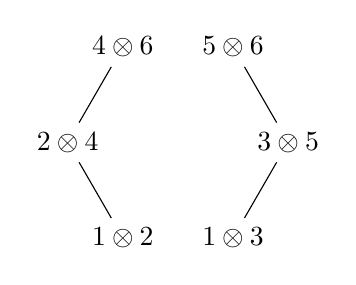
\begin{tikzpicture}[scale=.7]
  \node (one) at (60:2cm) {$5\otimes 6$};
  \node (b) at (120:2cm) {$4\otimes 6$};
  \node (a) at (180:2cm) {$2\otimes 4$};
  \node (zero) at (240:2cm) {$1\otimes 2$};
  \node (c) at (300:2cm) {$1\otimes 3$};
  \node (d) at (0:2cm) {$3\otimes 5$};
  \draw (zero) -- (a) -- (b);
  \draw (c)--(d)--(one);
\end{tikzpicture}
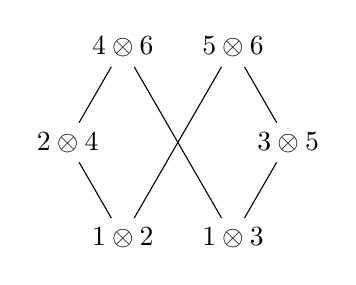
\begin{tikzpicture}[scale=.7]
  \node (one) at (60:2cm) {$5\otimes 6$};
  \node (b) at (120:2cm) {$4\otimes 6$};
  \node (a) at (180:2cm) {$2\otimes 4$};
  \node (zero) at (240:2cm) {$1\otimes 2$};
  \node (c) at (300:2cm) {$1\otimes 3$};
  \node (d) at (0:2cm) {$3\otimes 5$};
  \draw (zero) -- (a) -- (b) -- (c)--(d)--(one) -- (zero);
\end{tikzpicture}

Here, it is clear that $\mathcal F^1(P)$ is a graded poset, with $rk(x\otimes y) = rk(x),$ but, the hasse diagram on the right represents a poset which does not have a grading.
\end{counterexample}
\begin{proof}
\todo[inline]{prove this}
\end{proof}

We also have that the action of $G$ on $P$ induces an action on $\mathcal{F}^r(P)$ as follows.  

\begin{lem}\label{lem:G_action_on_FP}
The function defined by $g\cdot A = \{g\cdot a \colon a\in A\}$ for all $g\in G$, $A\in \mathcal{F}^r(P)$ is a well-defined group action of $G$ on $\mathcal{F}^r(P)$.
\end{lem}  

\begin{proof}
Since $g$ is an automorphism of $P$, $g\cdot A$ must also be isomorphic to $B_r$, that is $g\cdot A\in \mathcal{F}^r(P)$.  Suppose $A\le B$, and let $f\colon A\rightarrow B$ be an isomorphism satisfying $x\le f(x)$ for all $x\in A$.  Then $g\circ f\circ g^{-1}\colon g\cdot A \rightarrow g\cdot B$ is an isomorphism, and we have that $g^{-1}\cdot x \le f(g^{-1}\cdot x)$ by the definition of $f$.  Acting by $g$ on the left and using the fact that $g$ is order-preserving gives that $x\le g\cdot f(g^{-1}\cdot x)$, hence $g\cdot A\le g\cdot B$.  It follows that $g$ is an automorphism of $\mathcal{F}^r(P)$.
\end{proof}


\begin{prop}\label{prop:surjection_between_F_quotients}
For any group $G$ acting on $P$ and $0\le i\le \rk(P)$, we have $|\mathcal{F}^r(P/G)|_i \le |\mathcal{F}^r(P)/G|_i$. Furthermore there exists a poset surjection $q\colon \mathcal{F}^1(P)/G\rightarrow \mathcal{F}^1(P/G)$ defined by $q(G(x\otimes y)) = Gx\otimes Gy$, with $q$ being a bijection if and only if the action of $G$ on $P$ is cover transitive.\todo{maybe seperate out the cover transitive bit, and put it in the cover transitive section? I think it seems a bit out of place here}\todo{Can't we define cover transitive not only for $\mathcal F^1$, but also for $\mathcal F^r$? Wouldn't this theorem still hold exactly as stated for $\mathcal F^r$ with our new definition?}
\end{prop}

\begin{proof}
Let $Gx\otimes Gy\in \mathcal{F}^r(P/G)$.  Since the orbits between $Gx$ and $Gy$ form a boolean algebra of size $r$, it is possible to pick a set of representatives from the orbits in $Gx\otimes Gy$ such that the representatives form a boolean subalgebra $x\otimes y$ of size $r$ in $P$.  Then $x\otimes y\in \mathcal{F}^r(P)$ and the orbit $G(x\otimes y)$ is in $\mathcal{F}^r(P)/G$.  Furthermore, if $Gy^\prime\otimes Gx^\prime \ne Gy\otimes Gx$, then any boolean subalgebra $x^\prime\otimes y^\prime$ given by representatives from orbits lying between $Gx^\prime$ and $Gy^\prime$ will not be an element of $G(x\otimes y)$, since $(Gx,Gy)\ne (Gx^\prime,Gy^\prime)$.  Thus a choice of representatives from each boolean subalgebra of size $r$ in $\mathcal{F}^r(P/G)$ gives a rank-preserving injection $\mathcal{F}^r(P/G)\rightarrow \mathcal{F}^r(P)/G$ and hence $|\mathcal{F}^r(P/G)|_i \le |\mathcal{F}^r(P)/G|_i$.

Now consider the case when $r = 1$.  A boolean subalgebra of size 1 simply corresponds to an edge between adjacent ranks defined by a covering relation $x\lessdot y$ for some $x,y\in P$.  Then for every edge $x\otimes y\in \mathcal{F}^1(P)$, the orbit $Gx\otimes Gy$ is an element of $\mathcal{F}(P/G)$, so we get a map $q\colon \mathcal{F}^r(P)/G \rightarrow \mathcal{F}^1(P/G)$ by defining $q(G(x\otimes y)) = Gx\otimes Gy$.\todo{Elise:"which is clearly surjective"}  Note that this map is well defined because if $x^\prime\otimes y^\prime = g(x\otimes y) = g\cdot x\otimes g\cdot y$ for some $g\in G$, then $x^\prime\in Gx$ and $y^\prime\in Gy$.  Furthermore, we have that $G(x\otimes y) \le G(w\otimes z)$ if and only if there exist some $x_0\otimes y_0\in G(x\otimes y)$, $w_0\otimes z_0\in G(w\otimes z)$ such that $x_0\le w_0$ and $y_0\le z_0$.  If this is the case, then we also have that $Gx\otimes Gy \le Gw\otimes Gz$ by definition.

Finally, note that $q$ is a bijection exactly when there do not exist multiple\todo{Elise: maybe "distinct" instead of "multiple" would be clearer }orbits $G(x\otimes y) \ne G(x^\prime\otimes y^\prime)$ with $x^\prime\in Gx$, $y^\prime\in Gy$.  Fix $x\otimes y, x^\prime\otimes y^\prime\in \mathcal{F}^1(P)$ such that $x^\prime\in Gx$ and $y^\prime\in Gy$.  Pick a $g\in G$ such that $g\cdot y^\prime = y$.  Then $g\cdot x^\prime \otimes y\in G(x^\prime\otimes y^\prime)$, so $G(x\otimes y) = G(x^\prime \otimes y^\prime)$ if and only if there exists some $g^\prime\in G$ such that $g^\prime\cdot x = g\cdot x^\prime$ and $g^\prime\cdot y = y$. Hence $q$ is a bijection if and only if the $G$ action is cover transitive.
\end{proof}

\begin{counterexample}
In the previous theorem, we stated that $q$ is a bijection if and only if the action of $G$ on $P$ is cover transitive. However, it is {\it not} true that if the action of $G$ on $P$ is cover transitive, then $q$ is an isomorphism. A counterexample is provided as follows. Take $G=D_{20} \subset S_{10}$ acting by reflections and rotations on $[10]$ and hence acting on $B_{10}.$ We shall see in Lemma ~\ref{dihedral001} that this action is cover transitive. However, consider $x = \{2,4\},y = \{1,2,4\},a = \{2,4,7\},b = \{2,4,6,7\}.$ Then we may observe $x \otimes y,a \otimes b \in \mathcal F(B_{10})$ and $Gx < Ga, Gy < Gb,$ so $Gx \otimes Gy <_{\mathcal F^1(B_{10}/G} Ga \otimes Gb.$ However, it is not true that $G(x\otimes y)<_{\mathcal F^1(B_{10})/G} G(a\otimes b).$
\end{counterexample}

\section{The Poset $\mathcal{H}^r(P)$}
In this discussion we discuss a modified version of $\mathcal{F}^r(P)$, which we will denote $\mathcal{H}^r(P)$. The main point of introducing this object is to give a simple, noncomputational proof that $\mathcal F^r(B_n)/G$ is Peck. 

At least for the case $r=1$ there is an alternative proof of this fact. It is actually shown in Section ~\ref{sec:unitary_peck_f} that $\mathcal F^1(B_n)$ is unitary Peck, for $n>2,$ so, by Theorem \ref{thm:quotients_of_unitary_peck_posets}, $\mathcal F^1(B_n)/G$ is Peck. However, the proof of this is extremely messy and computational.

\todo{are we obligated to check whether $\mathcal F^r(B_n)$ is unitary Peck? Maybe we should at least put it as a question.}

We now define the object $\mathcal H^r(P),$ whose elements are the same as those of $\mathcal{H}^r(P),$ but we define a different partial order on $\mathcal{H}^r(P)$.

\begin{defn}
\label{defn:h_map}
For $P$ a graded poset, define the graded poset $\mathcal H^r(P)$ as follows. If $(x,y) \in P\times P,x <y,rk_P(x) + r = rk_P(y),$ then $x \otimes y \in \mathcal H^r(P).$ We declare $x\otimes y \lessdot_{\mathcal H} x' \otimes y'$ if $x \lessdot x',y\lessdot y'$ and $x' \not < y.$ Then, define $\leq_{\mathcal H}$ to be the transitive closure of $\lessdot_{\mathcal H}.$ Define $rk_{\mathcal H^r(P)}(x\otimes y) = rk_P(x).$
\end{defn}

\begin{warning}
While $\mathcal F^r:\mathcal P \rightarrow \mathcal P$ is a functor, $\mathcal H^r$ is not a functor. In particular, we have not specified how $\mathcal H^r$ acts on morphisms. If, for $f:P \rightarrow Q,$ we attempted to define $\mathcal H^r(f):\mathcal P \rightarrow \mathcal Q,$ we would quickly run into troubles. For example, suppose we took $f$ mapping a diamond $P$ (leftmost below) to a chain of length three $Q$ (second leftmost) Then, $\mathcal H^1(P)$ (second rightmost) has four points, with two pairs of edges, whereas $\mathcal H^1(Q)$ (rightmost) has two disconnected points. It is clear that there can be no order preserving mapping between these two objects. 

\begin{tikzpicture}[scale=.7]
  \node (b) at (0:2cm) {$3$};
  \node (a) at (90:2cm) {$4$};
  \node (c) at (180:2cm) {$2$};
  \node (d) at (270:2cm) {$1$};
  \draw (a) -- (b) -- (d) -- (c)--(a);
\end{tikzpicture}
\begin{tikzpicture}[scale=.7]
  \node (b) at (90:2cm) {$3$};
  \node (a) at (270:2cm) {$1$};
  \node (c) at (0:0cm) {$2$};
  \draw (a) -- (c) -- (b);
\end{tikzpicture}
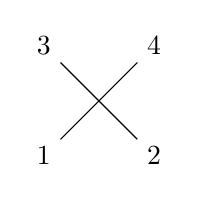
\begin{tikzpicture}[scale=.7]
  \node (b) at (45:1.414cm) {$4$};
  \node (a) at (135:1.414cm) {$3$};
  \node (c) at (225:1.414cm) {$1$};
  \node (d) at (315:1.414cm) {$2$};
  \draw (a) -- (d) ;
  \draw (c) -- (b);
\end{tikzpicture}
\begin{tikzpicture}[scale=.7]
  \node (b) at (90:1cm) {$2$};
  \node (a) at (270:1cm) {$1$};
\end{tikzpicture}
\todo{Put all pictures in figures, and make them look nicer}
However, it is still true that $\mathcal H^r(P)$ can be viewed as a graded poset with $rk_{\mathcal H^r(P)}(x\otimes y) = rk_P(x).$
\end{warning}

\todo{David, the proof of this lemma is the same as one that we need for $\mathcal F$ section, so you can probably put this proof there, and feel free to replace this proof by "similarly to the proof for F..."}
\begin{lem}\label{lem:HP_order}
For $P$ a graded poset, the object $\mathcal{H}^r(P)$, as defined in Definition ~\ref{defn:h_map} is a graded poset.
\end{lem}
\begin{proof}
To show $\mathcal H^r(P)$ is graded, we must show $x\otimes y <_{\mathcal H} a \otimes b \implies rk(x\otimes y)<rk(a \otimes b)$ and $x\otimes y \lessdot_{\mathcal H} a \otimes b \implies rk(x\otimes y)+1 = rk(a \otimes b).$ 

First, if $x\otimes y <_{\mathcal H} a \otimes b$ then by definition of $<_{\mathcal H},$ in Definition ~\ref{defn:h_map}, we must have $x < a,$ and hence 
$$rk_{\mathcal H^r(P)}(x\otimes y) = rk_P(x)<rk_P(a) = rk_{\mathcal H^r(P)}(a\otimes b).$$
Second, if $x\otimes y \lessdot_{\mathcal H} a \otimes b$ then $x \lessdot_P a,$ so $rk(x)+1 = rk(a)$ and then $$rk_{\mathcal H^r(P)}(x\otimes y)+1 = rk_P(x) +1=rk_P(a)= rk_{\mathcal H^r(P)}(a\otimes b).$$
\end{proof}

\begin{rem}\label{rem:order_containment}
Note that $x\otimes y\lessdot_{\mathcal{H}} a\otimes b \Rightarrow x\otimes y\lessdot_{\mathcal{F}} a\otimes b$.
\end{rem}

Similarly to $\mathcal{F}^r(P)$, the action of $G$ on $P$ induces an order-preserving action of $G$ on $\mathcal{H}^r(P)$.

\todo{David, once again, the proof of this Lemma is the same as one that we need for $\mathcal F$ section, so you can probably put this proof there, and feel free to replace this proof by "similarly to the proof for F..."}
\begin{lem}
\label{lem:G_action_on_HP}
The function defined by $g\cdot (x\otimes y)= gx\otimes gy$ for all $g\in G$, $x\otimes y\in \mathcal{H}^r(P)$ is a well-defined order preserving, rank preserving group action of $G$ on $\mathcal{H}^r(P)$.
\end{lem}

\begin{proof}
Clearly the action on $\mathcal H^r(P)$ is well defined because the action of $G$ on $P$ is. It is rank preserving because $$rk_{\mathcal H^r(P)}(g\cdot(x\otimes y)) = rk_{\mathcal H^r(P)}(gx\otimes gy)) = rk_P(gx)=rk_P(x) = rk_{\mathcal H^r(P)}(x\otimes y).$$
Finally, in order to show the action is order preserving, it suffices to show that if $x\otimes y \lessdot_{\mathcal H} a \otimes b$ then $g(x\otimes y) \lessdot_{\mathcal H} g(a \otimes b),$ because $\leq_{\mathcal H}$ is the transitive closure of $\lessdot_{\mathcal H}.$ By definition of $\lessdot_{\mathcal H},$ we have $x \lessdot a,y\lessdot b,y \not \leq b.$ Since the action of $G$ on $P$ is order preserving, it follows $gx \lessdot ga,gy \lessdot gb, gy \not \leq gb.$ This implies $gx\otimes gy \lessdot_{\mathcal H} ga \otimes gb = g(x\otimes y) \lessdot_{\mathcal H} g(a \otimes b).$
\end{proof}

\begin{prop}\label{prop:computing_HBn}
$\mathcal{H}^r(B_n)$ is isomorphic to $\binom{n}{r}$ disjoint copies of $B_{n-r}$.
\end{prop}

\begin{proof}

Suppose we have $x\otimes y,x'\otimes y' \in \mathcal H^r(B_n)$ with $x\otimes y \lessdot x'\otimes y'.$ Let $j\in [n]$ such that $y^\prime = y\cup\{j\}$, and let $i\in [n]$ such that $x^\prime = x\cup \{i\}$. If $i \ne j,$ then $x' \leq y,$ contradicting the assumption that $x\otimes y \lessdot_{\mathcal H} x'\otimes y'.$ Thus $x^\prime = x\cup\{i\}$ and $y^\prime = y\cup\{i\}$ for some $i\in [n]$.

Conversely we can easily check that if $i\not\in y$, then $x\otimes y\lessdot_{\mathcal{H}} x\cup\{i\}\otimes y\cup\{i\}$.  It follows that for all subsets $w\subset [n]$ such that $|w| = r$, there is an isomorphism from the subposet of elements $\{x\otimes y\colon y\setminus x = w\}$ to $B_{n-r}$ defined by $x\otimes y\mapsto (x\setminus w)\otimes (y\setminus w)$.  Furthermore if $y\setminus x \ne y^\prime \setminus x^\prime$, then $x\otimes y$ and $x^\prime\otimes y^\prime$ are incomparable, so these subposets indexed by $w$ are pairwise disjoint, and $\mathcal{H}^r(B_n)$ is isomorphic to $\binom{n}{r}$ copies of $B_{n-r}$.
\end{proof}



The primary advantage of Proposition \ref{prop:computing_HBn} is it allows us to easily see that $\mathcal{H}^r(B_n)$ is unitary Peck, which then implies that $\mathcal{H}^r(B_n)/G$ is Peck for any subgroup $G\subseteq S_n$.


\begin{cor}\label{cor:HBn_unitary_peck}
$\mathcal{H}^r(B_n)$ is unitary Peck for all $n\ge r$.
\end{cor}

\begin{proof}
This follows immediately from Proposition \ref{prop:computing_HBn} and the fact that $B_{n-r}$ is unitary Peck, as shown, for instance in \cite[Theorem 2a]{quotients_stanley} because $B_k = (B_1)^k$ and $B_1$ is clearly unitary Peck.
\end{proof}

\begin{cor}\label{cor:quotients_of_HBn_peck}
$\mathcal{H}^r(B_n)/G$ is Peck for any subgroup $G\subset S_n$.
\end{cor}

\begin{proof}
This follows from Corollary \ref{cor:HBn_unitary_peck} and Theorem \ref{thm:quotients_of_unitary_peck_posets}
\end{proof}

\begin{lem}
\label{lem:bijection_peck_implication}
If $f:P\rightarrow Q$ is a bijection and $P$ is Peck then $Q$ is Peck.
\end{lem}
\begin{proof}
Let $rk(P) = rk(Q) = n.$ Since $P$ is Peck, there exists an order raising map $U_i:P_i\rightarrow P_{i+1}$ such that $U_{n-i-1} \cdots U_i:P_i \rightarrow P_{n-i}$ is an isomorphism. Then, define $f(U)_i:P_i\rightarrow P_{i+1}$ by $f(U)_i(x) = f(U_i(f^{-1}(x))).$ This map is well defined because $f$ is a bijection. This map is order raising because $y > x \implies f(y) > f(x),$ by definition of morphisms of posets. It follows that since $U_{n-i-1} \cdots U_i$ is an isomorphism, $f(U)_{n-i-1} \cdots f(U)_i$ is as well, because the vector spaces $V(P_i) \cong V(Q_i)$ since $f$ is a bijection. Therefore, $Q$ is Peck.
\end{proof}

\begin{lem}
\label{bijection_h_f}
The map $f:\mathcal H^r(P) \rightarrow \mathcal F^r(P),G(x\otimes y) \mapsto G(x\otimes y)$ is a bijection.
\end{lem}
\begin{proof}
The elements of $\mathcal H^r(P),\mathcal F^r(P)$ are precisely the same by definition. Therefore, as long as $f$ is a morphism, it is automatically a bijection. Since $f$ is clearly rank preserving, to show $f$ is a morphism, it suffices to show $f$ is order preserving. This is immediate from Remark ~\ref{rem:order_containment}
\end{proof}

\begin{cor}
\label{cor:quotiented_edge_peck}
$\mathcal{F}^r(B_n)/G$ is Peck for any subgroup $G\subset S_n$.
\end{cor}
\begin{proof}
By Corollary ~\ref{cor:quotients_of_HBn_peck}, $\mathcal H^r(B_n)/G$ is Peck. By Lemma ~\ref{bijection_h_f}, the map $f:\mathcal H^r(P) \rightarrow \mathcal F^r(P),G(x\otimes y) \mapsto G(x\otimes y)$ is a bijection. Then, by Lemma ~\ref{lem:bijection_peck_implication}, it follows that $\mathcal F^r(B_n)/G$ is Peck.
\end{proof}

\subsection{A Generalization of $\mathcal H^r,\mathcal F^r$}
Although for the most part, we shall investigate $\mathcal F^1(P/G),\mathcal F^1(P)/G,$ there is a natural further generalization of $\mathcal H^r,$ to what we shall call $\mathcal H^{\vec r},$ where $\vec r = r_1,r_2,\ldots, r_k$ is an integer valued sequence. The results holding for these generalizations are analogous to those developed above. The purpose of developing these generalizations notion will be to give a more general application to Polya theory than could be given with $\mathcal H^r,$ for $r \in \BBZ$.

\begin{defn}
Let $\vec r = r_1,\ldots,r_k.$ For a graded poset $P,$ define the graded poset $\mathcal H^{r_1,\ldots, r_k}(P),$ also notated $\mathcal H^{\vec r}(P),$ whose elements are formal symbols $x_1 \otimes x_2 \otimes \cdots \otimes x_{k+1}$ such that $rk(x_i)+r_i = rk(x_{i+1}),$ for all $i \in [k].$ Say $x_1 \otimes x_2 \otimes \cdots \otimes x_{k+1}\lessdot_{\mathcal H^{\vec r}} y_1 \otimes y_2 \otimes \cdots \otimes y_{k+1}$ if $x_i \lessdot_P y_i,y_{i} \not \leq_P x_{i+1}$ for all $i \in [k+1].$ Then, define a relation $<_{\mathcal H^{\vec r}}$ on $\mathcal H^{r_1,\ldots, r_k}(P),$ to be the transitive closure of $\lessdot_{\mathcal H^{\vec r}}.$ Finally, define $rk_{\mathcal H^{\vec r}(P)}(x_1\otimes x_{k+1}) = rk_P(x_1)$
\end{defn}

\begin{defn}
Let $\vec r = r_1,\ldots,r_k,$ with $r_i \in \BN\forall i \in [k].$ Let $\mathcal P$ be the category of graded posets. Define the functor $\mathcal F^{\vec r}:\mathcal P \rightarrow \mathcal P,$ also notated $\mathcal F^{r_1,\ldots, r_k}.$ For a graded poset $P,$ define the graded poset $\mathcal F^{r_1,\ldots, r_k}(P),$ also notated whose elements are formal symbols $x_1 \otimes x_2 \otimes \cdots \otimes x_{k+1}$ such that $rk(x_i)+r_i = rk(x_{i+1}),$ for all $i \in [k].$ Say 
$x_1 \otimes x_2 \otimes \cdots \otimes x_{k+1}\lessdot_{\mathcal H^{\vec r}} y_1 \otimes y_2 \otimes \cdots \otimes y_{k+1}$ if $x_i \lessdot_P y_i$ for all $i \in [k+1]$. Then, define a relation $\leq_{\mathcal F^{\vec r}}$ on $\mathcal F^{r_1,\ldots, r_k}(P),$ to be the transitive closure of $\lessdot_{\mathcal F^{\vec r}}.$ Finally, define $rk_{\mathcal F^{\vec r}(P)}(x_1\otimes x_{k+1}) = rk_P(x_1)$
\end{defn}

\begin{rem}
Both $\mathcal F^{\vec r},\mathcal H^{\vec r}$ are functors, for the same reasons that $\mathcal F^r, \mathcal H^r$ are functors. This generalization is essentially taking the nerves of the poset $P.$ See \cite{babson} for some related constructions, although their constructions are different in many crucial ways.
\end{rem}

In the next Lemmas, we cite analogous results which hold for $\mathcal H^{\vec r}.$ The proofs are almost identical to those for $\mathcal H^r.$

\begin{lem}
Given a group action $\phi:G \times P \rightarrow P$ there are well defined group actions $\phi_{\mathcal F}:G\times \mathcal F^{\vec r}(P) \rightarrow \mathcal F^{\vec r}(P),\phi_{\mathcal H}:G\times \mathcal H^{\vec r}(P) \rightarrow \mathcal H^{\vec r}(P),$ 
both given by $g \cdot (x_1\otimes \cdots \otimes x_{k+1}) =g\cdot x_1 \otimes \cdots \otimes g \cdot x_{k+1}.$
\end{lem}
\begin{proof}
The proof is analogous to Lemma ~\ref{lem:G_action_on_HP}, Lemma ~\ref{lem:G_action_on_HP}.
\end{proof}

\begin{lem}
\label{lem:peck_quotients_vector_f}
The poset $\mathcal H^{r_1,\ldots, r_k}(B_n)$ is isomorphic to the multinomial coefficient $\binom n {r_1,r_2,\ldots, r_k}$ disjoint copies of $B_{n- \sum_{i=1}^k r_i}.$ Consequently, $\mathcal H^{\vec r}(B_n)$ is unitary Peck and $\mathcal H^{\vec r}(B_n)/G$ is Peck.
\end{lem}
\begin{proof}
Once again, the proof of the above three statements is analogous to those of ~\ref{prop:computing_HBn}, Corollary ~\ref{cor:HBn_unitary_peck}, and Corollary ~\ref{cor:quotients_of_HBn_peck}. The reason there are multinomial coefficients here instead of binomial coefficients, is that an element $x_1 \otimes x_2 \otimes \cdots \otimes x_{k+1}$ lies in the copy of $B_{n -\sum_{i=1}^k r_i}$ determined by the ordered tuple of subsets $(x_2 \setminus x_1,x_3 \setminus x_2, \ldots, x_{k+1} \setminus x_k).$ The first consists of $r_1$ elements, the next of $r_2$ elements, up through the last which consists of $r_k$ elements. Since the total number of ways to choose $r_1,\ldots, r_k$ in $k$ distinct groups is $\binom n {r_1,r_2,\ldots, r_k},$ there are exactly this many disjoint copies of $B_{n- \sum_{i=1}^k r_i}.$
\end{proof}

\section{Cover Transitive Actions}
\label{sec:cover_transitive}
In this section, we develop the theory of cover transitive actions $\phi$ where $G$ is a group, $P$ is a poset, and $\phi:G\times P \rightarrow P$ is an action. Recall Definition ~\ref{defn:cover_transitive}, that $\phi$ is cover transitive if whenever $x,y,z \in P,x\lessdot y,y\lessdot z,x \in Gy$ then there exists $g \in Stab(z)$ with $gx = y.$ For cover transitive actions $\phi:G\times P \rightarrow P,$ we shall show that, $\mathcal F^1(P/G)$ is Peck. Additionally, we shall show the cover transitive property is closed under semidirect products, in the appropriate sense. It is obvious that the action of $S_k$ on $B_k$ is cover transitive, and we shall also see in Lemma ~\ref{dihedral001} that the action of certain dihedral groups are cover transitive. We can then use these as building blocks to construct other cover transitive groups. In particular, we shall show in this section that automorphism groups of rooted trees are cover transitive.

\begin{eg}
\label{eg:trivial_edgequot}
Two rather trivial examples of cover transitive actions are $\phi:S_n\times B_n \rightarrow B_n,\psi:G\times B_n\rightarrow B_n$ where $G$ is arbitrary, $\phi$ is the permutation action and $\psi$ is the trivial action. In the former case, $\mathcal F^1(B_n/S_l)$ is simply a chain with $n-1$ points, and so is $\mathcal F^1(B_n)/S_l,$ since all $x\otimes y$ are identified under the $S_l$ action. In the latter case, since $G$ acts trivially by $\phi,$ both  $\mathcal F^1(B_n/G) \cong F^1(B_n)$ and $\mathcal F^1(B_n)/G \cong \mathcal F^1(B_n).$ So again, $\psi$ is cover transitive.

Developing less trivial examples will take a bit more work, but it will be shown in Lemma ~\ref{dihedral001} that Dihedral groups of order $2p$ and $4p$, for $p$ prime, are cover transitive.
\end{eg}

\begin{thm}
If an action $\phi:G \times P \rightarrow P$ is cover transitive, and $\mathcal F^1(P)$ is Peck, then $\mathcal{F}^1(P/G)$ is Peck.
\end{thm}
\begin{proof}
By Proposition ~\ref{prop:surjection_between_F_quotients}, there is a surjection $q:\mathcal F^1(P)/G \rightarrow \mathcal F^1(P/G).$ Additionally, by the same Proposition ~\ref{prop:surjection_between_F_quotients}, if $\phi$ is cover transitive, $q$ is a bijection. Finally, by Lemma ~\ref{lem:bijection_peck_implication}, since $q:\mathcal F^1(P)/G \rightarrow \mathcal F^1(P/G)$ is a bijection and $\mathcal F^1(P)/G$ is Peck, it follows that $\mathcal F^1(P/G)$ is Peck.
\end{proof}

In addition to the equivalent characterization of cover transitive actions as a bijection of posets, given in Proposition ~\ref{prop:surjection_between_F_quotients}, there is one more equivalent characterization of cover transitive actions, which is worth noting.

\todo{maybe write this as one of three equivalent conditions, together with q being a bijection}
\begin{lem}
\label{lem:upper_cover_transitive}
An action $\phi:G\times P \rightarrow P$ is cover transitive if and only if whenever $a<c,b<c, a \in Gb,$ there exists $h \in \Stab(c)$ with $ha = b.$
\end{lem}
\begin{proof}
Using Proposition ~\ref{prop:surjection_between_F_quotients}, $G$ is cover transitive if and only if the map $q$ defined in Proposition ~\ref{prop:surjection_between_F_quotients} is a bijection. However, $q$ is a bijection if and only if there do not exist distinct orbits $G(x\otimes y) \neq G(x'\otimes y')$ with $x' \in Gx,y'\in Gy.$ Fix $x \otimes y,x'\otimes y' \in \mathcal F^1(P)$ such that $x' \in Gx,y'\in Gy$. Choose $g \in G$ with $gx' = x.$ Then, $x' \otimes g\cdot y \in G(x'\otimes y').$ Since $g y' \in Gy,$ and $q$ is a bijection, the statement $x' \otimes g\cdot y \in G(x'\otimes y')$ is equivalent to $G(x'\otimes y') = G(x\otimes y).$ This, in turn is equivalent to the existence of $g' \in G$ with $g'x = x,g'y = gy'.$ Then, taking $a = x,b = y,c = gy',h = g',$ the existence of such a $h=g'\in G$ is equivalent to the statement that whenever $a<c,b<c, a \in Gb,$ there exists $h \in \Stab(c)$ with $ha = b,$ as we wanted to show.
\end{proof}


\ssec{Preservation Under Direct Products}
\label{ssec:direct_product_preservation}

\begin{thm}
\label{thm:direct_product_preservation}
For $\phi:G\times P\rightarrow P,\psi:H \times Q \rightarrow Q$ two cover transitive actions, then the direct product $\phi \times \psi:(G\times H)\times (P\times Q) \rightarrow (P\times Q),(g,h)\cdot (x,y) \mapsto (gx,hy)$ is also cover transitive.
\end{thm}
\begin{proof}
For every element $x\in P\times Q$ write $x = (x_G,x_H)$, where $x_G \in P, x_H \in Q.$. Suppose $a < c$, $b < c$ for some $a,b,c\in P\times Q$ such that there exists some $(g,h)\in G\times H$ with $(g,h)\cdot a = b$. Then $a_G < c_G$, $b_G < c_G$, and $g\cdot a_G = b_G$, so there exists some $g^\prime \in G$ such that $g^\prime\cdot c_G = c_G$ and $g^\prime\cdot a_G = b_G$ since $\phi$ is cover transitive.  Similarly there exists some $h^\prime \in H$ such that $h^\prime \cdot c_H = c_H$ and $h^\prime a_H = b_H$.  Then $(g^\prime,h^\prime)\cdot c = c$ and $(g^\prime,h^\prime)\cdot a = b$, so $\phi\times \psi$ is cover transitive as desired.
\end{proof}
\ssec{Preservation Under Wreath Products.}
\label{ssec:wreath_preservation}

Next, we turn our attention to proving that if $\psi:G \times P \rightarrow P$ is cover transitive, we can naturally construct an action $\phi:(G\wr S_l)\times P^l \rightarrow P^l$ is also cover transitive. This is shown in Theorem ~\ref{thm:wreath_preservation}

\begin{defn}
For $G, H$ groups, with $H \subset S_l,$ the {\it wreath product}, notated $G \wr H,$ is the group whose elements are pairs $(g,h) \in G^l\times H$ with multiplication defined by
\begin{align*}
((g_1',\ldots, g_l'),h') \cdot ((g_1,\ldots, g_l) ,h) =((g'_{h'(1)}g_1,\ldots, g'_{h'(l)}g_l),hh')
\end{align*}
where $h \in H$ acts on $[l]$ by the restriction of the permutation action of $S_l$ to $H.$
\end{defn}

In other words, $G\wr H$ can be viewed as a certain semidirect product of $G^l \rtimes H.$

\begin{note}
\label{note:wreath_action}
For any group $G$ with a given action $\psi:G\times P \rightarrow P,$ we obtain an induced action of $G \wr H,$ $\phi:G \wr H \times P^l \rightarrow P^l$ defined by 
$$((g_1,\ldots, g_l),h)(a_1,\ldots, a_l) = (g_{h^{-1}(1)}\cdot a_{h^{-1}(1)},\ldots,g_{h^{-1}(l)} \cdot a_{h^{-1}(l)}).$$
\end{note}

\begin{rem}
Heuristically, one may think of the above action as obtained by first having $G$ act separately on the $l$ distinct copies of $P,$ and then letting $H$ act by permuting the copies.
\end{rem}

\begin{thm}
\label{thm:wreath_preservation}
If $\psi:G\times P \rightarrow P$ is cover transitive, then $\phi:G\wr S_l \times P^l \rightarrow P^l$ where $\phi$ is the induced action defined in Notation ~\ref{note:wreath_action} is also cover transitive.
\end{thm}
\begin{proof}

Notate an element $y = (y_1,\ldots, y_l)$ where $y_i$ lies in copy $i$ of $P,$ inside $P^l.$ Suppose we have $a \otimes c \in \mathcal F^1(P^l)$ and $b \in Ga,b < c.$ The aim is to show there exists $(g,h) \in \Stab_{G\wr S_l}(c)$ with $(g,h)a = b.$ 

Since $a \lessdot c, b \lessdot c$ there must be a unique $i \in [l]$ with $a_i \lessdot c_i,$ and for all other $k,k\neq i,a_k = b_k.$ Similarly, there is a unique $j \in [l]$ with $b_j \lessdot c_j$ and for all other $k,k\neq j,b_k = c_k.$ We may assume $i \neq j$  because if $i = j,$ then since $G$ is cover transitive, we can find $g' \in G$ with $g'(a_i) = b_i,g' \in \Stab(c_i).$ Then, taking $g \in G^n$ so that $g_i = g'$ and $g_k = \id$ for $k \neq i,$ then $(g,\id)a = b,(g,\id) \in \Stab(b),$ as desired.

Next, because $a \in (G\wr S_l)b,$ it must be that the multisets $\{(G \wr S_l)a_1,\ldots, (G \wr S_l)a_l\}=\{(G \wr S_l)b_1,\ldots, (G \wr S_l)b_l\}$ are equal. However, we know that for all $k \neq i,j$ $a_k = b_k$. Therefore, there is an equality of multisets $\{(G \wr S_l)a_i,(G \wr S_l)a_j\} = \{(G \wr S_l)b_i,(G \wr S_l)b_j\}.$ However, since $a_i \lessdot c_i = b_i$ and $a_j = c_j \gtrdot b_j,$ and since the $G\wr S_l$ action is rank preserving, it follows that $(G \wr S_l)b_j=(G \wr S_l)a_i, (G \wr S_l)a_j = (G \wr S_l)b_i.$

Define $\sigma \in S_l$ to be the permutation switching only $(i,j)$ and keeping all other elements fixed. Then, since $(G \wr S_l)a_j = (G \wr S_l)b_i,$ we may write $b_i = \sigma\delta a_j.$ 
Note that $\sigma \delta b_i = \delta \sigma b_i,$ where we view $\delta$ as an element of two different copies of $G$ inside $G \wr S_l.$ Then,
Since $\sigma \delta a_j = b_i,$ both $a_i \subset b_i,\sigma \delta b_j \subset b_i$ and additionally $\delta\sigma b_j = \sigma\delta b_j \in Ga_i.$ Therefore, since $G$ is cover transitive, there exists $\epsilon \in \Stab(c)$ with $\epsilon(\delta\sigma b_j) = a_i.$

Finally, define $g \in G^n$ with $g_j = \delta,g_i = \sigma\delta^{-1}\epsilon$ and for $k \neq i,j,g_k = \id.$ Then, by construction, $(g,\sigma) \in \Stab (c)$ and $(g,\sigma)a = b.$ Therefore, $\phi$ is cover transitive.
\end{proof}

\ssec{An application to rooted trees.}
\label{ssec:rooted_trees}
In this subsection, we prove that the automorphism group of rooted trees is always cover transitive. To do this we will apply Theorem ~\ref{thm:wreath_preservation} and Theorem ~\ref{thm:direct_product_preservation}, since the automorphism group of rooted trees is essentially built from direct products and wreath products with a symmetric group. To this aim, we first give definitions relating to rooted trees, then characterize their automorphisms, and finally show that such automorphism groups are always cover transitive.

\begin{defn}
A poset $P$ is a {\it rooted tree} if $P$ is a graded poset, there is a unique element $x \in P$ of maximal rank, called the {\it root}, and for all $x \in P,$ other than the root, there exists a unique $y \in P$ with $y \gtrdot x.$
\end{defn}

\begin{defn}
For $P$ a rooted tree, an element $x \in P$ is a {\it leaf} if there is no $z \in P$ with $x > z.$ Denote the set of all leaves of $P$ by $L(P).$
\end{defn}

\begin{lem}
\label{lem:induced_tree_action}
Let $P$ be a rooted tree and let $L(P)$ be the set of leaves of $P.$ Then, the action of $Aut(P)$ on $P$ induces an action of $Aut(P)$ on $L(P).$ Furthermore, there is also an induced action of $Aut(P)$ on $B_n$ where $n = |L(P)|.$ 
\end{lem}
\begin{proof}
First, we must show that $Aut(P)$ induces an action on $L(P).$ To show this, it suffices to show that for any $g \in Aut(P),x \in L(P),$ then $gx \in L(P).$ This fact, however, is easy to see, because if $gx \notin L(P),$ then there exists $y < gx.$ However, then $g^{-1}y < x,$ contradicting the assumption that $x$ is a leaf. We then obtain the induced action $Aut(P)\times L(P) \rightarrow L(P),(g,x)\mapsto gx.$

To complete the proof, we just have to give the induced action of $Aut(P)$ on $B_n.$ To do this, identify $L(P) \cong [n]$ as sets, where $|L(P)| = n$ by assumption. Then, for $g \in Aut(P),\{l_1,\ldots, l_k\} \in B_n,$ the induced action of $Aut(P)$ on $B_n$ is given by $g\{l_1,\ldots, l_k\} = \{g\cdot l_1,\ldots, g\cdot l_k\}.$
\end{proof}

\begin{convention}
For the rest of this section only, fix a rooted tree $P$ and denote by $G$ the group of automorphisms $Aut(P).$ Let $G$ act on $B_n,$ where $n = |L(P)|$ by the induced action $\phi:G \times P \rightarrow P,$ defined in the proof of Claim ~\ref{lem:induced_tree_action}.
\end{convention}

\begin{note}
For $x \in P,$ denote $D(x) = \{y \in P| y \leq x\}.$
\end{note}
\begin{prop}
\label{prop:automorphism_trees}
Let $P$ be a rooted tree with root vertex labeled $r$. Then, if let $\{A_1,\ldots,A_m\}$ denote the set of isomorphism classes of $\{D(x)|x\lessdot r\}.$ For $T \in A_j,$ denote $G_j = Aut(T).$ Then, 
\begin{equation}
\label{eq:level_expansion}
Aut(P) = (G_1 \wr S_{i_1}) \times (G_2 \wr S_{i_2}) \times \cdots \times (G_m\wr S_{i_m}),
\end{equation}
In particular, $Aut(P)$ can be expressed as a sequence of direct products and wreath products of symmetric groups.
\end{prop}

\begin{proof}
It is clear that if $P$ is rank 1, with $|P_0| = n,$ then the automorphism group is $S_n.$ So, let us proceed by induction. That is, label the vertices of $P$ by $\{0,1,\ldots, s\}$ such that the root is labeled $0$ and the vertices just below the root are labeled $1, \ldots, k.$ Let $A_1,\ldots, A_m$ denote the distinct isomorphism classes of trees in the set $\{D(1),\ldots, D(k)\}.$ For $T \in A_j,$ denote $G_j = Aut(T).$ 
Let $T_j = \{t|t\lessdot 0,t \in A_j\}.$ Then, letting $Q_j$ be the subtree of $P$ whose elements lie in the set $0 \cup (\cup_{t \in T_j} D(t)),$ it follows $Aut(Q_j) \cong G_j \wr S_{i_j},$ because after choosing a permutation of the elements of $T_j,$ we are free to choose any element of $G_j$ to permute each $D(t),t \in T_j$. If $t_1 \lessdot 0,t_2 \lessdot 0,g \cdot t_1 = t_2,$ then it must be that $D(t_1) = D(t_2).$ Therefore, $Aut(P)$ must permute these isomorphism classes of trees, and the full automorphism groups is simply the direct product, 
\begin{equation}
\label{eq:level_expansion}
Aut(P) = (G_1 \wr S_{i_1}) \times (G_2 \wr S_{i_2}) \times \cdots \times (G_m\wr S_{i_m}),
\end{equation}
Since each $G_j$ is a sequence of direct products and wreath products with symmetric groups by the inductive assumption, it follows from ~\eqref{eq:level_expansion} that so is $Aut(P).$
\end{proof}

\begin{cor}
For $P$ the automorphism group of a rooted tree, $Aut(P)$ is cover transitive.
\end{cor}
\begin{proof}
First, the permutation action $\phi:S_n \times B_n \rightarrow B_n$, is clearly cover transitive, as was noted in Example ~\ref{eg:trivial_edgequot}. By Theorem ~\ref{thm:wreath_preservation}, wreath products with symmetric groups preserve the cover transitive property, and by Theorem ~\ref{thm:direct_product_preservation} the direct product of two cover transitive groups is again cover transitive. Therefore, by Proposition ~\ref{prop:automorphism_trees}, all groups of the form $Aut(P)$ are built up from these operations, and so $Aut(P)$ is also cover transitive.
\end{proof}

\section{Wreath Product of two Symmetric Groups}

In this section,we prove a result similar to that of \cite[Theorem 1.1]{pak}. We shall construct a certain sequence which is not only unimodal, but can even be exhibited as the ranks of a Peck poset. It shall give an alternate proof of Theorem 1.1 in the case that $r = 1.$

\begin{note}
We shall now show 
For this section, fix $l,m$ with $n = l \cdot m$ and fix $G = S_m \wr S_l.$ Let $S_m$ act on $B_m$ by the permutation representation, and then let $G$ act on $B_{m}^l\cong B_{m \cdot l}$ by the action defined in Notation ~\ref{note:wreath_action}.
\end{note}

\ssec{Recalling Pak and Panova's Result}
We first review the necessary definitions and then state \cite[Theorem 1.1]{pak}:

A {\it partition} is a sequence of numbers $\lambda = (\lambda_1,\ldots, \lambda_k)$ such that $\lambda_1 \geq \lambda_2 \geq \cdots \geq \lambda_k.$ If $\sum_{i=1}^k \lambda_i = n$ then $\lambda$ is a {\it parition of $n$}, notated $\lambda \vdash n.$ A {\it composition} is a sequence of numbers $\lambda = (\lambda_1,\ldots, \lambda_k).$ That is, it is a partition where order matters. If $\sum_{i=1}^k \lambda_i = n$ then $\lambda$ is a {\it composition of $n$}. Let $P_n(l,m)$ denote the set of partitions $\lambda = (\lambda_1,\ldots, \lambda_k) \vdash n,$ such that $\lambda_1 \leq m,k \leq l.$ That is, $P_n(l,m)$ is the partitions which fit inside an $l \times m$ rectangle.

\begin{note}
\cite[Section 1]{pak} For $\lambda$ a partition, let $\nu(\lambda)$ be the number of distinct nonzero part sizes of $\lambda.$
\end{note}

\begin{note}
\cite[Section 1]{pak}
Let $p_k(l,m,r) = \sum_{\lambda \in P_k(l,m)} \binom{\nu(\lambda)}{r}.$
\end{note}

\begin{thm}
\label{thm:pak_thm}
\cite[Theorem 1.1]{pak}
The sequence $p_r(l,m,r), p_{r+1}(l,m,r),\ldots, p_{l\cdot m}(l,m,r)$ is unimodal and symmetric.
\end{thm}

\ssec{The Poset $\mathcal F^r(B_n)/G$}
Now that we have managed to state Pak and Panova's Theorem, we will begin the trek toward showing how the $p_1(l,m,1)$ are actually ranks of $\mathcal F^1(B_n/G).$ The first step is to describe the Peck poset $\mathcal F^1(B_n)/G.$ In particular, we shall obtain an explicit formula for the sizes of its ranks in Theorem ~\ref{thm:quotiented_edge_wreath}. To do this, we will first describe representatives for the vertices of $B_n/G$ and then analogous representatives for vertices of $\mathcal F^1(B_n)/G.$

\begin{defn}
For $x \subset [l \cdot m]$ we shall say $x$ is {\it left justified} if whenever $a \in x,$ such that $a \neq 1 \pmod l,$ then $a -1 \in x.$ In other words, when we pick out the boxes of the $l\times m$ rectangle which lie in $x$ the resulting diagram is left justified.
\end{defn}

\begin{defn}
For $x \subset [l\cdot m],$ define the {\it composition of $x,$} denoted $comp(x) = \lambda_1 ,\ldots, \lambda_l$ where $\lambda_i = |\{a \in x|i\cdot (m-1)< a \leq i \cdot m\}|.$ That is, if we pick out the boxes of the $l \times m$ rectangle which lie in $x,$ the composition is just the sequence of the number of boxes in each row. Similarly, define the {\it partition of $x$,} notated $part(x)$ as follows. Let $\pi \in S_l$ be a permutation such that $\pi(i) \geq \pi(i+1)$ for all $i,1\leq i \leq l-1.$ Then  $part(x) = (\lambda_{\pi(1)},\ldots, \lambda_{\pi(l)}).$ That is, $part(x)$ is the $comp(x)$, written in decreasing order.
\end{defn}

\begin{lem}
\label{lem:comp_invariance}
For any $g \in G, x \in B_n,$ it follows that $part(x) = part(gx).$
\end{lem}
\begin{proof}
It suffices to show this holds for any generator $g.$ Then. $G$ is generated by elements which permute rows, and elements that swap rows. It is clear that if $g$ only permutes elements in a single row, then $comp(gx) = comp(x)$, so in particular, $part(gx) = part(x).$ If $g$ swaps two rows, then $comp(gx)$ is simply a reordering of the parts of $comp(x)$, and so again $part(gx) = part(x).$
\end{proof}

\begin{defn}
For $x \subset [l\cdot m],$ say $x$ is a {\it Young Diagram} if $x$ is left justified and $comp(x)$ is a partition.
\end{defn}

\begin{lem}
\label{lem:young_diag_reps}
For each $x \in B_{l\cdot m}$ there exists a unique representative $z \in Gx$ such that $z$ is a Young Diagram.
\end{lem}
\begin{proof}
Uniqueness is clear, because for any $g \in G,$ by Claim ~\ref{lem:comp_invariance}, $part(gx) = part(x).$ So, to we only have to show there is some $g \in G$ for which $gx$ is a Young Diagram. Indeed, first, choose $h_1 \in G$ so that $h_1x$ is left justified. This can be done because every permutation of a single row in the $l\times m$ rectangle lies in the wreath product, so, we can take $h_1$ to be the product of the elements that left justify each individual row. Then, let $h_2$ be the element that swaps the rows of $h_1x$ so that they increase going down. Finally, taking $g = h_2 h_1,$ it follows that $gx$ is a Young diagram. 
\end{proof}

\begin{note}
For $x \in B_n$ denote by $\overline{x}$ the unique element in $Gx$ such that $\overline{x}$ is a Young Diagram.
\end{note}

Now that representatives for each $G$ orbit in $B_n$ have been described, we shall move on to describing representatives for each $G$ orbit in $\mathcal F(B_n).$

\begin{note}
For $\lambda = (\lambda_1,\ldots, \lambda_k)$ a partition, introduce the alternate notation $\lambda = a_1^{b_1} \cdots a_s^{b_s}$ if the first $b_1$ parts of $\lambda$ are equal to $a_1,$ the next $b_2$ parts of $\lambda$ are equal to $b_2$, and in general, for $1 \leq h\leq b_j$, the parts $ \lambda_{h+\sum_{i=1}^{j-1} b_i}$ are all equal to $a_j.$ Furthermore, all $a_j$ must be distinct.
\end{note}

\begin{lem}
\label{lem:young_diag_reduction}
If $x\otimes y, w \otimes y \in\mathcal F^r(B_n)_i$ then $x\otimes y \in G(w \otimes y)$ if and only if for all $g \in G$ such that $gy$ is a Young diagram, we have $gx \otimes gy \in G(gw \otimes gy).$ In particular, if $gy = \overline y$ then $x\otimes y \in G(w\otimes y)$ if and only if $gx \otimes \overline y \in gw \otimes \overline y.$
\end{lem}
\begin{proof}
Clearly $g(x\otimes y) \in G(g(w\otimes y))$ if and only if $x \otimes y \in G(w \otimes y).$
\end{proof}

The point of the proceeding Lemma is that in order to determine when two elements are identified, we may assume that $y$ is a young diagram.

\begin{note}
For $y$ a Young Diagram with $part(y) = comp(y) = a_1^{b_1}\cdots a_s^{b_s},$ and $x \subset y,$ for all $i,1 \leq i \leq s,$ define $y_i$ to be the $a_i \times b_i$ rectangle consisting of the rows $1+\sum_{j = 1}^{i-1} b_j,2+\sum_{j = 1}^{i-1} b_j,\ldots, \sum_{j = 1}^{i} b_j.$ That is, $y_i$ is just the rectangle of all parts of $y$ which are of length $a_i.$
\end{note}

\begin{prop}
\label{prop:wreath_orbits}
If $y$ is a Young Diagram so that $part(y) = comp(y) =a_1^{b_1}\cdots a_s^{b_s}$, and $x\otimes y, w \otimes y \in\mathcal F^r(B_n)_j$ then $x\otimes y \in G(w \otimes y)$ if and only if for all $i,1 \leq i \leq s,$ it holds that $part(x\cap y_i) = part(w \cap y_i).$
\end{prop}
\begin{proof}
First, suppose for all $i,1 \leq i \leq s,$ that $part(x\cap y_i) = part(w\cap y_i).$ We know both $x\subset y, w \subset y$. Further, since $y_i$ is a rectangle, there exists some $g \in \Stab(y_i)$ so that $gx = w.$ Then, for each $i,$ there exists some $g_{1,i} \in \Stab(y_i)$ so $g_{1,i}(x \cap y_i)=\overline{x \cap y_i},$ which only interchange elements in $y_i.$ Similarly, there exists $g_{2,i} \in \Stab(y_i),g_{2,i}(w \cap y_i) = \overline{w\cap y_i}.$ However, the assumption $part(x\cap y_i) = part(w\cap y_i)$ precisely means $\overline{x \cap y_i}= \overline{w\cap y_i}.$ Therefore, $g_{2,i}^{-1}g_{1,i} \in \Stab(y)$ and $g_{2,i}^{-1}g_{2,i}(x \cap y_i) = (w \cap y_i).$ Applying this same procedure for all $i$ and multiplying the corresponding group elements together gives an element $g \in \Stab(y)$ with $gx = w.$ Therefore, $g(x\otimes y) = gx \otimes gy = gx \otimes y = w \otimes y,$ so $x\otimes y \in G(w \otimes y).$

Conversely, note that $x\otimes y \in G(w \otimes y)$ is equivalent to the existence of a $g \in \Stab(y)$ with $gx = w.$ However, any $g \in \Stab(y)$ can only interchange rows of the same length. Therefore, we obtain the stronger result that we can write $g = h_1 \cdots h_s$ where $h_i \in \Stab(y_i),$ and $h_i(p) = p$ for all $p \notin y_i.$ Then, it follows that $h_i(x \cap y_i) = w \cap y_i$ and so $part(x\cap y_i) = part(w\cap y_i),$ as claimed.
\end{proof}

\begin{rem}
So, one way of viewing $G$ orbits of an element $x \otimes y \in \mathcal F^r(B_n)$ is as ``outer'' Young Diagrams, made up of a sequence of rectangles stacked on top of one another, each one wider than the next, which form the Young diagram $\bar y.$ Then, to each such rectangle we associate an ``inner'' Young Diagram. The inner young diagram corresponds to the elements in that rectangle in $y$ but not in $x.$ Two elements are in the same $G$ orbit if and only if their ``outer'' Yound Diagram and ``inner'' Young Diagrams are all the same.
\end{rem}

The next step is to give explicitly formulas for the ranks of $\mathcal F^r(B_n).$

\begin{note}
For $p(x) = \sum_{i=0}^N c_ix^i,$ a polynomial, define the notation $[p(x)]_r = c_r.$
\end{note}

Now, we briefly introduce notation for $q$ binomial coefficients, so that we can state the next propositions. Let $q \in \BR$ and let $[n]_q = \sum_{i=0}^{n-1} q^i.$ Then, denote $[n]_q! = \prod_{i=1}^n [i]_q.$ Finally, let $\binom n k_q = \frac{[n]_q!}{[k]_q![n-k]_q!}.$

\begin{note}
For $\lambda = (a_1^{b_1} \cdots a_s^{b_s})$ a partition, denote $\eta(\lambda,r) = \left[\prod_{i=1}^s \binom{a_i+b_i}{a_i}_q\right]_r.$
\end{note}

\begin{prop}
\cite[Proposition 1.3.19]{enumerative_comb}
\label{prop:counting_box_partitions}
There is an equality $[\binom {a+b} b_q]_j = |P_j(l,m)|.$
\end{prop}

\begin{thm}
\label{thm:quotiented_edge_wreath}
The sizes of the ranks of $\mathcal F^r(B_n)/G$ can be written as 
$$|(\mathcal F^r(B_n)/G)_i| = \sum_{\lambda \in P_i(l,m)} \eta(\lambda,r).$$
\end{thm}
\begin{proof}

By Proposition ~\ref{prop:wreath_orbits} each orbit $x \otimes y$ has a representative such that $y$ is a Young Diagram, with $part(y) = \prod_{i=1}^s a_i^{b_i},$ and each $x \cap y_i$ is a Young Diagram. Therefore, for a fixed $y,$ the number of orbits $x \otimes y$ with $|x|+r = |y|$ is exactly determined by the Young Diagrams of $\overline{x \cap y_i},$ for $1 \leq i \leq s.$ Equivalently, it is determined by the Young Diagrams $[y_i \setminus x],$ for $1 \leq i \leq s.$ So, we wish to calculate the number of tuples of Young Diagrams of the form $(\overline{y_1 \setminus x},\overline{y_2 \setminus x},\ldots, \overline{y_s \setminus x})$ so that $\sum_{i=1}^s |y_i \setminus x| = r.$ Now, define $j_i$ by $j_i = |y_i \setminus x|,$ still of course with, $\sum_{i=1}^s j_i = r.$ Then, by Proposition ~\ref{prop:counting_box_partitions}, the number of such partitions is $[\binom {a_i+b_i} {b_i}_q]_{j_i}.$ Therefore, the number of elements $G(x\otimes y)$ with $j_i = |y_i \setminus x|,$ is simply the product $\prod_{i=1}^s [\binom {a_i+b_i} {b_i}_q]_{j_i}.$ Therefore, since $j_i$ were chosen arbitrarily, only subject to the constraint that $\sum_{i=1}^s j_i = r,$ It follows that the total number of elements $G(x\otimes y),$ for $y$ fixed, is equal to 
\begin{align*}
\sum_{\substack{{(j_1,\ldots, j_s),}\\{\sum_{i=1}^s j_i = r}}} \prod_{i=1}^s \left[\binom {a_i+b_i} {b_i}_q\right]_{j_i} = \left[\prod_{i=1}^s \binom {a_i+b_i} {b_i}_q\right]_{r} = \eta(\lambda,r).
\end{align*}
Then, summing this over all Young Diagrams $y,$ gives that

\begin{align*}
|\mathcal F^r(B_n)/G|_i = \sum_{\lambda \in P_i(l,m)}  \left[\prod_{i=1}^s \binom {a_i+b_i} {b_i}_q\right]_{r} = \sum_{\lambda \in P_i(l,m)} \eta(\lambda,r).
\end{align*}

\end{proof}



\todo{the following commented out section was based on the old definition of $\mathcal F^r$. Should we remove it?}

\iffalse

\ssec{The poset $\mathcal F(B_n/G).$} Now that we understand $\mathcal F(B_n/G),$ we turn our attention to understanding $\mathcal F(B_n/G).$ Then, we look at how the two relate, and draw some interesting consequences. But first, we have to characterize representative elements of $\mathcal F(B_n/G),$ and the size of its ranks.

\begin{lem}
\label{lem:pairs_in_edge_poset}
Let $x,y \in (B_n)_i$ with $part(y)= a_1^{b_1}\cdots a_s^{b_s}.$ Then, for two orbits $Gx,Gy,$ with $|x|+1=|y|,$ we have that $Gx \otimes Gy \in \mathcal F^r(B_n/G)$ if and only if there exist distinct indices $i_1,\ldots, i_r$ such that $|x\cap y_{i_t}|+1 = |y_{i_t}|$ for $1 \leq t \leq r,$ and otherwise  $|x\cap y_{i_t}|= |y_{i_t}|.$
\end{lem}
\begin{proof}
By definition, $Gx\otimes Gy\in \mathcal F^r(B_n/G)_i$ if and only if the set of orbits $Gz$ with $Gx \leq Gz \leq Gy$ is isomorphic to the hypercube $B_r.$ Choosing representatives $\overline{x},\overline{y}$ which are Young Diagrams for $Gx,Gy,$ we now wish to describe the Young Diagrams $\overline{z}$ with $\overline{x} \subset \overline{z} \subset \overline{y}.$ If $(\overline{y}\setminus \overline{x}) \cap \overline{y}_i \leq 1$ for all $i,$ then such $z$ are precisely given by choosing any subset of $S \subset \{i_1,\ldots, i_r\}$, and taking $\overline{z} = S \cup x.$ Clearly such $z$ form a hypercube $B_r.$

Conversely, if there is some $i$ for which $(\overline{y}\setminus \overline{x}) \cap y_i > 1,$ we will show there are strictly fewer than $2^r$ Young Diagrams $\overline{z}$ with $\overline{x}\subset \overline{z} \subset \overline{y}.$ In particular, this will imply the set of elements between then cannot be isomorphic to $B_r.$ There are clearly at most $2^r$ such intermediate diagrams, as described above, given by choosing any subset of $S \subset \{i_1,\ldots, i_r\}$, and taking $\overline{z} = S \cup x.$ Therefore, it suffices to show there are two subsets $S_1,S_2$ with $\overline{x}\cup S_1 \in G(\overline{x}\cup S_2).$ To produce these two subsets, suppose $a,b \in (\overline{y}\setminus \overline{x}) \cap \overline{y}_i$ for some $i$. There exists such an $i$ with $a \neq b$ by assumption. Then, taking $S_1 = \{a\},S_2=\{b\}$ gives us that $\overline{x}\cup S_1 \in G(\overline{x}\cup S_2)$ because we can take $g \in \Stab(y_i)$ so that $S_1 = gS_2.$
\end{proof}

\begin{thm}
\label{thm:edge_of_quotiented_wreath}
The size $|\mathcal F^r(B_n/G)|_i = \sum_{\lambda \in P_i(l,m)} \binom{\nu(\lambda)} r.$
\end{thm}
\begin{proof}
Fix an orbit $Gy$ and its corresponding Young Diagram $\overline{y},$ with $part(y) = a_1^{b_1}\cdots a_s^{b_s}.$ Of course, here $s = \nu(part(y)).$ Then, by Lemma ~\ref{lem:pairs_in_edge_poset}, any element $Gx \otimes Gy \in \mathcal F^r(B_n/G)$ must have that $|x| +r = |y|$ and $|(y \setminus x)\cap y_i| \leq 1.$ The number of such elements is precisely the number of ways of choosing $r$ distinct part sizes from $y.$ In particular there are $\binom{\nu(part(y))} r$ such elements $\overline{x} \otimes \overline{y}.$ Therefore, summing this over all Young Diagrams $y$ yields
\begin{align*}
|\mathcal F^r(B_n/G)|_i = \sum_{\lambda \in P_i(l,m)} \binom{\nu(\lambda)} r.
\end{align*}
\end{proof}
\fi
\ssec{Ensuing Conclusions}
We now reap the fruits of our labor in order to draw some nice results.

\iffalse
I think we will not need the following, thanks to some work in above sections.
\begin{lem}
\label{lem:wreath_1_isom}
There is an isomorphism of vector spaces $$V(F^1(B_{l\cdot m}/G))_i \cong V(\mathcal F^1(B_{l\cdot m})/G)_i$$ for all $i.$
\end{lem}
\begin{proof}
By Proposition ~\ref{prop:surjection_between_F_quotients}, there is a surjection $V(\mathcal F^r(B_{l\cdot m}/G)_i \rightarrow V(F^r(B_{l\cdot m})/G)_i$ for all $i.$ Hence, in order to prove these posets are isomorphic, it suffices to show they have the same dimension. However, by the proof of Theorem ~\ref{thm:quotiented_edge_wreath} shows that in the case $r = 1,\eta(\lambda,1)$ is equal to the number of Young Diagrams $x$ of size $i-1$ contained in $y.$ This is clearly equal to $\nu(\lambda)$ since such young diagrams $x$ are exactly those given by removing a corner of $y.$ Therefore, $\eta(\lambda,1) = \nu(\lambda).$ Therefore, $\sum_{\lambda \in P_i(l,m)} \eta(\lambda,1) = \sum_{\lambda \in P_i(l,m)} \binom{\nu(\lambda)} r.$

Finally, using this observation, together with both of Theorem ~\ref{thm:quotiented_edge_wreath}, and Theorem ~\ref{thm:quotiented_edge_wreath}, 
\begin{align*}
|\mathcal F^r(B_{l\cdot m})/G|_i =\sum_{\lambda \in P_i(l,m)} \eta(\lambda,1) = \sum_{\lambda \in P_i(l,m)}\nu(\lambda) = |F^r(B_{l\cdot m}/G)|_i.
\end{align*}
Hence,  $\dim V(\mathcal F^r(B_{l\cdot m}/G))_i = \dim V(F^r(B_{l\cdot m})/G)_i,$ so in particular, the surjection from Proposition ~\ref{prop:surjection_between_F_quotients} is an isomorphism.
\end{proof}

\begin{cor}
\label{cor:peck_wreath_1}
The poset $\mathcal F^1(B_{l\cdot m}/G)$ is Peck.
\end{cor}
\begin{proof}
Since $G = S_m \wr S_l,$ and the permutation action of $S_m$ on $B_m$ is cover transitive, by ...
\end{proof}

This result was based on the old definition of $\mathcal F^r.$

\begin{cor}
The poset $\mathcal F^r(B_{l\cdot m}/G)$ is symmetric and unimodal for all $r.$
\end{cor}
\begin{proof}
By Theorem ~\ref{thm:pak_thm}, the sequence $p_r(l,m,r), p_{r+1}(l,m,r),\ldots, p_{l\cdot m}(l,m,r)$ is unimodal and symmetric, and by Theorem ~\ref{thm:edge_of_quotiented_wreath}, $|\mathcal F^r(B_n/G)_i| = p_i(m,l,r).$
\end{proof}

\fi

\begin{cor}
\label{cor:unimodal_wreath_r_sequence}
The sequence $\sum_{\lambda \in P_r(l,m)} \eta(\lambda,r),\ldots,\sum_{\lambda \in P_n(l,m)} \eta(\lambda,r),$ is the sequence of ranks of the Peck poset $\mathcal F^r(B_{l\cdot m})/G.$ In particular, the sequence is symmetric and unimodal.
\end{cor}
\begin{proof}
By Theorem ~\ref{thm:quotiented_edge_wreath}, $\sum_{\lambda \in P_i(l,m)} \eta(\lambda,r)$ is the size of the $i-r$th rank of the Peck poset $\mathcal F^r(B_{l\cdot m})/G.$ Since Peck posets are unimodal and symmetric, this sequence is as well.
\end{proof}

We now obtain an easy proof of Theorem ~\ref{thm:pak_thm} for the case $r = 1.$ Using the fact that $S_m\wr S_l$ is cover transitive. Namely,

\begin{cor}
\label{cor:rank_gen_fn_wreath_1}
The sequence $p_1(l,m,1), p_{r+1}(l,m,1),\ldots, p_{l\cdot m}(l,m,1)$ is the rank generating function of $\mathcal F^1(B_{l\cdot m})/G.$ In particular, the sequence is unimodal and symmetric.
\end{cor}
\begin{proof}
First, we know $F^1(B_{l\cdot m})/G$ is Peck, since it is the quotient of a unitary Peck poset by a group action. However, it is easy to see that $\eta(\lambda,1) = \nu(\lambda),$ since both count the number Young Diagrams of size $|\lambda|-1$ fitting inside the Young Diagram corresponding to $\lambda.$ Therefore, $\sum_{\lambda \in P_i(l,m)} \eta(\lambda,r) = \sum_{\lambda \in P_i(l,m)}\nu(\lambda) = p_i(l,m,1).$ However, by Corollary ~\ref{cor:unimodal_wreath_r_sequence}, $\sum_{\lambda \in P_r(l,m)} \eta(\lambda,r),\ldots,\sum_{\lambda \in P_n(l,m)} \eta(\lambda,r),$ are the ranks of $\mathcal F^1(B_{l\cdot m})/G.$ Therefore, $p_i(l,m,1)$ are also the ranks of $\mathcal F^1(B_{l\cdot m})/G$, hence symmetric and unimodal.
\end{proof}

\section{An Application to Polya Theory}
\label{sec:polya}
In this section, we use the generalized notion of $\mathcal H^{\vec r}(B_n)$ to obtain the unimodality of the coefficients a certain class of polynomials from Polya Theory, which will turn out to be the rank generating function of $\mathcal H^{\vec r}(B_n)/G.$ The result we prove is a generalization of \cite[Corollary 7.16]{algebraic_stanley}. 

\ssec{A Brief Review of Polya Theory}

We shall follow the treatment from \cite[Chapter 7]{algebraic_stanley}. First, we build up some definitions to state Polya's Theorem.

\begin{defn}
Let $G \subset S_n$ act on $[n]$ by the restriction of the permutation action. For $\pi \in G,$ the action of $\pi$ on $[n]$ can be written in cycle notation so that there are $c_i$ cycles of length $i.$ Define the {\it cycle indicator} of $\pi$ to be the monomial $Z_\pi(z_1,\ldots, z_n) = z_1^{c_1}z_2^{c_2}\cdots z_n^{c_n}.$
\end{defn}

\begin{defn}
The {\it cycle indicator} for a group $G \subset S_n,$ is the polynomial $$Z_G(z_1,\ldots, z_k) = \frac{1}{|G|}\sum_{\pi \in G} Z_\pi(z_1,\ldots, z_k).$$
\end{defn}

\begin{defn}
A {\it coloring} of a set $S$ by the colors $R = \{r_1,\ldots, r_k\}$ is a map $S \rightarrow R.$ Heuristically, a coloring of $S$ can be thought of as an assignment of a ``color'' from the set $R$ to each of the elements of $S.$
\end{defn}

\begin{note}
For $A,B$ sets, let $A^B = Hom_{\text{sets}}(B,A).$ Let $G \subset S_n$ act on $B_n.$ Then, $G$ acts on $R^{B_n} = Hom_{\text{sets}}(B_n,R)$ by $g \cdot f(S) = f(g\cdot S)$ where $g \in G,S \in B_n, f \in R^{B_n}.$ Then, let $R^{B_n}/G$ denote the quotient of $R^{B_n}$ by the action of $G$ defined above.

For $f \in R^{S},$ say $color(f) = (i_1,\ldots, i_k)$ if $|\{s \in S|f(s) = j\}| = i_j$ for $1 \leq j \leq k.$ Observe that if $f \in Gh$ then $color(f) = color(h),$ so the map $color$ descends to a map on $G$ orbits.

Define $\kappa(i_1,\ldots, i_k) = |\{Gf \in R^{B_n}/G \text{ such that } color(f) = (i_1,\ldots, i_k) \}|.$

Finally, let $F_G(r_1,\ldots, r_k) = \sum_{i_1,\ldots, i_k} \kappa(i_1,\ldots, i_k)r_1^{i_1} \cdots r_k^{i_k}.$
\end{note}

\begin{rem}
The above notation may seem extremely cumbersome. It is simply a formal way of saying that $\kappa(i_1,\ldots, i_k)$ is the number of inequivalent colorings of subsets of $B_n,$ under the $G$ action. Once again, see \cite[Chapter 7]{algebraic_stanley} for a more lengthy exposition.
\end{rem}

\begin{thm}
\label{thm:polya}
(Polya's Theorem)
Let $G \subset S_n$ act on $B_n.$ With $F_G,Z_G$ as defined above, the following equality holds.
$$F_G(r_1,\ldots, r_k) = Z_G(\sum_{i=1}^k r_i,\sum_{i=1}^k r_i^2,\ldots, \sum_{i=1}^k r_i^n).$$
\end{thm}


\ssec{A Rank Generating Function}


\begin{note}
Let $[f(x_1,\ldots, x_k)]_{x_{j_1}^{i_1}\cdots x_{j_l}^{i_l}}$ denote the coefficient of $x_{j_1}^{i_1}\cdots x_{j_l}^{i_l}$ in $f(x_1,\ldots, x_k),$ which may itself be a polynomial.
\end{note}

\begin{lem}
\label{lem:polya_faces_equivlence}
The number $\kappa(i_1,\ldots, i_k)$ is equal to $|(\mathcal F^{i_2,\ldots, i_{k-1}}(B_n)/G)_{i_1}|.$ Consequently, 

$$[Z_G(\sum_{i=1}^k r_i,\sum_{i=1}^k r_i^2,\ldots, \sum_{i=1}^k r_i^n)]_{r_1^{i_1} \cdots r_k^{i_k}}=|(\mathcal F^{i_2,\ldots, i_{k-1}}(B_n)/G)_{i_1}|.$$
\end{lem}
\begin{proof}
Define a map $m:(F^{r_2,\ldots, r_{k-1}}(B_n))_{i_1} \rightarrow \{f \in R^{B_n}|color(f) =(i_1,\ldots, i_k)\}$ as follows. For $x_2 \otimes\cdots\otimes x_{k} \in \mathcal F^{r_2,\ldots, r_{k-1}}(B_n),$ let $m(x_2 \otimes\cdots\otimes x_{k}) = f,$ where 
$$f(t) = \begin{cases} r_1 &\text{ if } t\in x_2\\
r_i &\text{ if } t \in x_{i+1}\setminus x_i\\
r_k &\text{ if } t \notin x_k
\end{cases}.$$
Observe that $m$ is infact a bijection, as we can easily define an inverse map by sending a coloring $f$ to $x_2\otimes\cdots\otimes x_{k},$ where $x_j$ is the set of all elements $t \in [n]$ for which $f(t) = r_l,l<j,$ for all $j \in [k-1].$ 
Next, the two group actions were precisely defined so that so that, 
$$g(x_1\otimes x_{k-1}) = g(y_2 \otimes \cdots \otimes y_{k-1}) \iff g\cdot m(x_1\otimes x_{k-1}) = g\cdot m(y_2 \otimes \cdots \otimes y_{k-1})$$
Therefore, $m$ descends to a bijection $m^G:(F^{r_2,\ldots, r_{k-1}}(B_n))_{i_1}/G \rightarrow R^{B_n}/G,$ This implies $\kappa(i_1,\ldots, i_k)$ is equal to $|(\mathcal F^{i_2,\ldots, i_{k-1}}(B_n)/G)_{i_1}|.$ 

Then, by Polya's Theorem ~\ref{thm:polya},  
$$[Z_G(\sum_{i=1}^k r_i,\sum_{i=1}^k r_i^2,\ldots, \sum_{i=1}^k r_i^n)]_{r_1^{i_1} \cdots r_k^{i_k}}=\kappa(i_1,\ldots, i_k)=|(\mathcal F^{i_2,\ldots, i_{k-1}}(B_n)/G)_{i_1}|.$$
\end{proof}

Now we arrive at our main result of the section. The following result provides a rank generating function for $\mathcal F^{\vec r}(B_n)/G$

\begin{prop}
\label{prop:rank_gen_fn}
Let $z_j = \sum_{l = 1}^k r_l^j.$ Let $$Z_G^{i_2,\ldots,i_{k-1}}(r_1) =[Z_G(z_1,\ldots, z_{k-1},1)]_{r_2^{i_2}\cdots r_{k-1}^{i_{k-1}}},$$ be a polynomial in $r_1.$ Then, the coefficients of $Z_G^{i_2,\ldots,i_{k-1}}(r_1)$ are the ranks of the peck poset  $\mathcal F^{i_2,\ldots, i_{k-1}}(B_n)/G.$ In particular, they form a symmetric, unimodal sequence.
\end{prop}
\begin{proof}
In Lemma ~\ref{lem:polya_faces_equivlence}, we saw $$[Z_G(z_1,\ldots, z_k)]_{r_1^{i_1} \cdots r_k^{i_k}}=|(\mathcal F^{i_2,\ldots, i_{k-1}}(B_n)/G)_{i_1}|.$$
However, since $\sum_{j = 1}^k i_j = n,$ it follows that $i_k$ is determined by the numbers $i_1,\ldots, i_{k-1},$ and so 
$$[Z_G(z_1,\ldots, 1)]_{r_1^{i_1} \cdots r_k^{i_k}}=|(\mathcal F^{i_2,\ldots, i_{k-1}}(B_n)/G)_{i_1}|.$$
Next, write $Z_G^{i_2,\ldots,i_{k-1}}(r_1),$ defined in the statement of the Theorem, as $\sum_{t} c_t (r_1)^t.$ We have just shown that $c_t = |(\mathcal F^{i_2,\ldots, i_{k-1}}(B_n)/G)_{i_1}|.$ Since $\mathcal F^{i_2,\ldots, i_{k-1}}(B_n)/G$ is a Peck poset by Lemma ~\ref{lem:peck_quotients_vector_f}, its rank sizes form a symmetric and unimodal sequence. Therefore, the coefficients of $Z_G^{i_2,\ldots,i_{k-1}}(r_1)$ form a symmetric, unimodal sequence.
\end{proof}

\begin{rem}
Note that in the case $\vec r = 0,$ the above result precisely becomes \cite[Corollary 7.16]{algebraic_stanley}.
\end{rem}

\section{Further Identities for the Wreath Product}
In this section, we draw on the methods developed earlier in this section to write down some interesting generating functions for the case that $G = S_m \wr S_l.$
First, we shall use Proposition ~\ref{prop:rank_gen_fn} to obtain an explicit generating function for $p_i(l,m,1),$ and then we shall relate the sum $\sum_{\pi \in G} \binom{\Fix(\pi)}{t}$ to the $t$th Bell number, using $\mathcal F^{\vec r}(B_n)/G,$ where $\vec r$ is of the form $\vec r = 1,\ldots, 1$.

\begin{note}
For this section only, firx $m,l \in \BN$ and fix $G = S_m \wr S_l.$ Additionally, fix $n = m \cdot l.$
\end{note}

\ssec{A Generating Function for $p_i(l,m,1).$}

\begin{prop}
Let $c_i$ be the number of $i$ cycles in $\pi$ and define $$W_\pi(z_1,\ldots, z_n) = \begin{cases}\frac {Z_\pi(z_1,\ldots,z_n)}{z_1} &\text{ if } c_1 > 0 \\
0 &\text{ if } c_1 = 0
\end{cases}.$$

Then, there is an equality
$$\sum_{i=0}^n p_i(l,m,1) r_1^ir_2^{n-i-1} = \sum_{\pi \in G} |\Fix(g)|W_\pi(r_1 + r_2,r_1^2+r_2^2,\ldots,r_1^n + r_2^n).$$
\end{prop}
\begin{proof}
Recall from Corollary ~\ref{cor:rank_gen_fn_wreath_1} that $p_i(l,m,1)$ was the rank generating function of $\mathcal F^1(B_{l\cdot m})/G$. 

As was seen in Proposition ~\ref{prop:rank_gen_fn}, it is also the case that $$[Z_G(r_1+r_2+r_3,\ldots, (r_1)^n+(r_2)^n+(r_3)^n)]_{(r_3)^1}$$ is also the rank generating function of $|(\mathcal F^{1}(B_n)/G)_{i_1}|.$
Therefore, 
$$p_i(l,m,1)=[Z_G(r_1+r_2 + r_3,\ldots, r_1^n+ r_2^n + r_3^n)]_{r_3}.$$
So, to complete the proof, it suffices to show 
$$[Z_G(r_1+r_2 + r_3,\ldots, r_1^n+ r_2^n + r_3^n)]_{r_3} = \sum_{\pi \in G} |\Fix(g)|W_\pi(r_1 + r_2,r_1^2+r_2^2,\ldots,r_1^n + r_2^n).$$

To show this, it further suffices to show that for all $\pi \in G,$
$$Z_\pi(r_1+r_2 + r_3,\ldots, r_1^n+ r_2^n + r_3^n)]_{r_3} =  |\Fix(\pi)|W_\pi(r_1 + r_2,r_1^2+r_2^2,\ldots,r_1^n + r_2^n).$$

Indeed, this is easy to see, because for $r_3$ to have a nonzero coefficient in the expansion of $r_3$ in $Z_\pi,$ first, $\pi$ must have some 1-cycle, as otherwise, no variable could appear in the expansion of $Z_\pi$ raised only to the first power. Second, if $\pi$ has some 1-cycle, then the coefficient of $r_3$ in $$Z_\pi(r_1 + r_2+r_3,r_1^2+r_2^2+r_3^2,\ldots,r_1^n + r_2^n+r_3^n) = \prod_{i=1}^n (r_1^i+r_2^i+r_3^i)^{c_i}$$ is precisely 
$$c_1 \cdot W_\pi(r_1 + r_2,r_1^2+r_2^2,\ldots,r_1^n + r_2^n) = |\Fix(\pi)|W_\pi(r_1 + r_2,r_1^2+r_2^2,\ldots,r_1^n + r_2^n)$$ because $c_1$ is the number of 1-cycles in $\pi,$ which is by definition the number of fixed points of $\pi.$ This is exactly what we wanted to show.
\end{proof}

\ssec{Bounded Partition Sizes}
This section is an application of Polya theory, and is moderately tangential to the rest of the paper. However, it relates to the functor $\mathcal F^{\vec r},$ in that it counts the $|(\mathcal F^{\vec r}(B_n)/G)_0| =  |(\mathcal F^{\vec s}(B_n)/G)_1|,$ as described in Remark ~\ref{rem:box_partitions_relation_to_f}.

\begin{note}
Let $P_{[t]}[l,m]$ denote the set of partitions of the set $[t]$ into at most $l$ sets, such that each set in the partition has size at most $m.$ Let $P[l,m] = \cup_{t \in \BN} P_{[t]}[l,m]$ be the set of all partitions into at most $l$ sets such that each set in the partition has size at most $m.$ Denote $p_{[t]}[l,m] = |P_{[t]}[l,m]|,$ and $p[l,m] = |P[l,m]|.$
\end{note}

\begin{prop}
\label{prop:box_partition_by_size}
There is an equality $p_{[t]}[l,m] = \frac {t!}{l!(m!)^l}\sum_{\pi \in G} \binom {\Fix(\pi)} t.$
\end{prop}
\begin{proof}
Using Polya's Theorem ~\ref{thm:polya}, we know 
$$F_G(r_1,\ldots, r_k) = \frac 1 {|G|}Z_G(\sum_{i=1}^k r_i,\sum_{i=1}^k r_i^2,\ldots, \sum_{i=1}^k r_i^n).$$ In particular, 
$$[F_G(r_1,\ldots, r_k)]_{r_1 r_2 \cdots r_t r_{t+1}^{m\cdot l-t}} = [\frac 1 {|G|}Z_G(\sum_{i=1}^k r_i,\sum_{i=1}^k r_i^2,\ldots, \sum_{i=1}^k r_i^n)]_{r_1 r_2 \cdots r_t r_{t+1}^{m\cdot l - t}}.$$

Of course, by definition of $F_G,$ we know 
$$[F_G(r_1,\ldots, r_k)]_{r_1 r_2 \cdots r_t r_{t+1}^{m\cdot l-t}} = \kappa(1,1,\ldots, 1,m \cdot l - t,0,\ldots, 0)$$
where there are $t$ 1's in the above expression. By definition $\kappa$ is just the number of inequivalent ways to distinctly color $t$ numbers in an $l \times m$ rectangle, up to the action of $G = S_m \wr S_l.$ For any such coloring, let square $a_i$ be colored with color $r_i.$ Each $G$ orbit of colorings has a unique representative where along each row the colors are sorted in increasing order, and additionallly, going down the first column, the colors are sorted in increasing order. Here, we are basically ignoring color $t+1,$ just viewing it as a placeholder to color the remaining squares of the grid. Then, the colorings defined above are in bijection with partitions of $[t]$ so that this partition has at most $l$ sets, and each set in this partition has at most $m$ elements. The set of such partitions is exactly  $P_{[t]}[l,m].$ Therefore, the number of such partitions is $p_{[t]}[l,m].$ Then, it follows that
$$p_{[t]}[l,m] = \kappa(1,1,\ldots, 1,m \cdot l - t,0,\ldots, 0) = [\frac 1 {|G|}Z_G(\sum_{i=1}^k r_i,\sum_{i=1}^k r_i^2,\ldots, \sum_{i=1}^k r_i^n)]_{r_1 r_2 \cdots r_t r_{t+1}^{m\cdot l - t}}.$$

Of course, $\frac 1 {|G|} = \frac 1 {l!(m!)^l}$ when $G = S_m \wr S_l.$ So, to complete the proof, we just need to show that 
$$[Z_G(\sum_{i=1}^k r_i,\sum_{i=1}^k r_i^2,\ldots, \sum_{i=1}^k r_i^n)]_{r_1 r_2 \cdots r_t r_{t+1}^{m\cdot l - t}} =  t!\sum_{\pi \in G} \binom {\Fix(\pi)} t.$$

This follows from the definition of $Z_G.$ That is, it is the sum over all the cycle indicators $\sum_{\pi \in G}Z_\pi(\sum_{i=1}^k r_i,\sum_{i=1}^k r_i^2,\ldots, \sum_{i=1}^k r_i^n).$ So, to show the above holds, it suffices to show that
$$[Z_\pi(\sum_{i=1}^k r_i,\sum_{i=1}^k r_i^2,\ldots, \sum_{i=1}^k r_i^n)]_{r_1 r_2 \cdots r_t r_{t+1}^{m\cdot l - t}} =  t! \binom {\Fix(\pi)} t$$
This is now apparent, because $Z_\pi = \prod_{i < m \cdot l} (\sum_j r_j^i)^{c_i},$ where $c_i$ is the number of $i$ cycles in $\pi.$ The only way we can obtain a monomial of the form $r_1 r_2 \cdots r_t r_{t+1}^{m\cdot l - t}$ is if $c_1 > t.$ Then, the coefficient of such a term will exactly be the number of ways to choose an ordered set of $t$ elements from $c_1$ terms. That is, it is precisely $t!\binom {c_1} t.$ However, $c_1$ is the number of 1-cycles, that is $c_1 = \Fix(\pi).$ Hence, $[Z_\pi(\sum_{i=1}^k r_i,\sum_{i=1}^k r_i^2,\ldots, \sum_{i=1}^k r_i^n)]_{r_1 r_2 \cdots r_t r_{t+1}^{m\cdot l - t}} =  t!\binom {\Fix(\pi)} t$ as desired.
\end{proof}

\begin{rem}
\label{rem:box_partitions_relation_to_f}
Thanks to Proposition ~\ref{prop:rank_gen_fn}, an equivalent way to state the above result is that $\sum_{\pi \in G} \binom {\Fix(\pi)} t = |(\mathcal F^{\vec r}(B_n)/G)_0|,$ if $\vec r$ is the vector consisting of $t$ ones. Also, letting $\vec s$ be the vector with $t-1$ ones, we may note $ |(\mathcal F^{\vec r}(B_n)/G)_0| =  |(\mathcal F^{\vec s}(B_n)/G)_1|,$ since one may think of elements of 
$\mathcal F^{\vec s}(B_n)/G$ as tuples of $t-1$ elements, each contained in the next, whose lowest element is of rank 1, and one may think of elements of $(\mathcal F^{\vec r}(B_n)/G)_0$ as tuples of $t$ elements, each contained in the next, whose lowest element is of rank 0. There is an obvious bijection between these two sets, given by adding or removing the element $\emptyset$ or rank 0 in $B_n.$ Therefore, we also obtain $\sum_{\pi \in G} \binom {\Fix(\pi)} t = |(\mathcal F^{\vec s}(B_n)/G)_1|.$
\end{rem}

We can also get a formula for the size of the whole set $p[l,m]:$

\begin{prop}
\label{prop:all_box_partitions}
Define the function $f:\BN \cup 0 \rightarrow \BN,$ by $$f(x) = \begin{cases} \lfloor e\cdot n!\rfloor &\text{ if } n > 0 \\ 1 &\text{ if } n = 0\end{cases}.$$
Then, $$p[l,m] = \frac 1 {l!(m!)^l}\sum_{\pi \in G} f(|\Fix(\pi)|).$$
\end{prop}
\begin{proof}
First, note that $\sum_{i=1}^k i! \binom k i = f(k).$ This can be seen fairly easily, because $\sum_{i=1}^k i! \binom k i = k!\sum_{i=0}^k \frac 1 {i!},$ while $k! \cdot e = k!\sum_{i=0}^\infty \frac 1 {i!},$ and for $k > 1,$ it is easy to bound the difference $\sum_{i=k+1}^\infty \frac 1 {i!} < \frac 1 {k!},$ which implies   $\sum_{i=1}^k i! \binom k i  = \lfloor k! \cdot e \rfloor = f(k)$ for $k > 1.$

By definition, $p[l,m] = \sum_{t = 0}^{l\cdot m} p_{[t]}(l,m)$. Therefore, by Proposition ~\ref{prop:box_partition_by_size},
\begin{align*}
p[l,m] &= \sum_{t = 0}^{l\cdot m} p_{[t]}(l,m)\\
&=\sum_{t = 0}^{l\cdot m}\frac {t!}{l!(m!)^l}\sum_{\pi \in G} \binom {\Fix(\pi)} t\\
&= \frac {1}{l!(m!)^l}\sum_{t = 0}^{l\cdot m}\sum_{\pi \in G} t!\binom {\Fix(\pi)} t\\
&=  \frac {1}{l!(m!)^l}\sum_{\pi \in G}\sum_{t = 0}^{l\cdot m} t!\binom {\Fix(\pi)} t\\
&= \frac {1}{l!(m!)^l}\sum_{\pi \in G}\sum_{t = 0}^{l\cdot m} f(|\Fix(\pi)|).
\end{align*}
\end{proof}
\todo{Perhaps also put in the recursive relations which the $P[l,m]$ satisfy}

\section{Groups of order $n.$}

In this section, we shall show that for any group $G$ such that $|G| = n,$ with an order-preserving, rank preserving, transitive action on $B_n$, then $|\mathcal F^1(B_n)/G)_i| = \binom {n-1}{i-1}$ Any such action can be described by identifying $[n] \cong G,$ and then having $G$ act on itself by the left multiplication. We can then use a simple result in group theory to calculate the ranks of $\mathcal F^1(B_n)/G$ for all transitive actions $\phi:G\times P \rightarrow P,$ where $G$ is abelian.

For the rest of this section, fix a group $G$ with $|G| = n,$ and a transitive action of $G$ on $[n],$ which induces an action of $G$ on $B_n.$

\begin{lem}
\label{lem:stabilizer_one}
For $G$ a group acting transitively on $[n],$ it follows that $\Stab(x) = \{e\}.$
\end{lem}
\begin{proof}
Since $G$ acts transitively on $n$ we have the number of orbits $|[n]/G| = 1,$ Therefore, using Burnside's Lemma, together with the observation that $e \in \Stab(x)$,
$$|G| = \sum_{x\in X}|\Stab(x)|\geq \sum_{x \in X} 1=|X|= |G|.$$
Then, the above string of inequalities tells us that we must have $|\Stab(x)| = 1$ for all $x,$ or in other words, $\Stab(x) = \{e\}.$
\end{proof}

\begin{prop}
\label{prop:stabilizer_edge}
For any element $x \otimes y \in \mathcal F^1(B_n),$ then $\Stab(x\otimes y) = e.$
\end{prop}
\begin{proof}
From Lemma ~\ref{lem:stabilizer_one} for any $x \in B_n$ with $|x| = 1,$ we have $\Stab(x) = \{e\}.$ Then, by definition $\Stab(x\otimes y) = \Stab(x) \cap \Stab(y) = \Stab(x) \cap \Stab(y \setminus x).$ However, $\Stab(y \setminus x)$ is by assumption a 1 element set, because $|y| = |x| +1,x \subset y.$ This implies that $\Stab(x\otimes y)=\Stab(x) \cap \Stab(y \setminus x) = \Stab(x) \cap \{e\} = \{e\},$ for all $x \otimes y \in \mathcal F^1(B_n),$ as claimed.
\end{proof}

\begin{lem}
\label{lem:q_counts}
The number $|(\mathcal F^1(B_n)/G)_i| = \binom{n-1}{i}.$
\end{lem}
\begin{proof}
Since there are $\binom{n}{i}$ elements $x\in(B_n)_i,$ each with $n-i$ elements $y \in (B_n)_{i+1}$ with $x \subset y,$ there are a total of $\binom{n}{i}\cdot (n-i)$ elements $x \otimes y \in \mathcal F^r(B_n)_i.$ By Proposition ~\ref{prop:stabilizer_edge}, we have $|\Stab(x \otimes y)| = 1.$ Therefore, by the Orbit Stabilizer Theorem, it follows $|G(x\otimes y)| = n.$ So, all orbits have the same size. From this,
\begin{align*}
|\mathcal F^1(B_n)_i/G| = |\mathcal F^1(B_n)_i|/|G| = \frac{\binom{n}{i}\cdot (n-i)}{n} = \binom {n-1}{i}.
\end{align*}
\end{proof}

\begin{lem}
\label{lem:faithful_action}
For $G$ a group let $H \subset G$ be the subgroup such that $hx = x$ for all $x \in X,h \in H.$ Then, $H$ is a normal subgroup of $G$ and if $|G/H| = n,$ then $\mathcal F^1(B_n)/G =\mathcal F^1(B_n)/(G/H).$
\end{lem}
\begin{proof}
First, we check $H$ is normal. For any $g \in G,x \in x$ it follows $ghg^{-1}x = gh(g^{-1}x) = g(g^{-1}x) = (gg^{-1})x = x$, and so $ghg^{-1} \in H.$ Hence, $G/H$ is a group.

Then, observe $Gx = (G/H)x$ because $H$ acts trivially. Therefore, $\mathcal F^1(B_n)/G \cong \mathcal F^1(B_n)/(G/H),$ since $G,G/H$ have exactly the same orbits.
\end{proof}

\begin{lem}
\label{lem:transitive_abelian}
All faithful transitive abelian groups $A$ acting on the set $[n]$ have $|A| = n.$
\end{lem}
\begin{proof}
This is a well known, easy to prove, result. See for instance \cite{stack}
\end{proof}

\begin{cor}
\label{cor:transitive_abelian_ranks}
Any abelian group $A$ which acts transitively on $[n]$ has $|\mathcal F (B_n)/A|_i= \binom{n-1}{i}.$
\end{cor}
\begin{proof}
By Lemma ~\ref{lem:faithful_action}, we can assume $A$ acts faithfully as well.
By Lemma ~\ref{lem:transitive_abelian}, $|A| = n.$ Then, by Lemma ~\ref{lem:q_counts}, $|\mathcal F (B_n)/A|_i = \binom{n-1}{i}.$
\end{proof}






\section{Quotient by the Cyclic Group}
\label{sec:cyclic}

In this section, we show that for $G = C_n$ the cyclic group of order $n$, the poset $\mathcal F^1(B_n/G)$ is rank symmetric and rank unimodal. The rank symmetric part is obvious. From Corollary ~\ref{cor:transitive_abelian_ranks}, we know that for $G = C_n$, the size of the $i^{th}$ rank of the poset $\mathcal F^1 (B_n)/C_n$ is $$|\mathcal F^1 (B_n)/C_n|_{i} = \binom{n-1}{i}.$$
We will bound $|\mathcal F^1(B_n/C_n)|_{i}$ by  $|\mathcal F^1 (B_n)/C_n|_{i}$ to obtain the unimodality. 


\begin{note} Throughout the section, we fix an arbitrary $n$ to start with, and set $$q_i = |\mathcal F^1 (B_n)/C_n|_{i}, \quad p_i = |\mathcal F^1(B_n/C_n)|_{i}. $$
\todo{ $ |\mathcal F^1(B_n/C_n)|_{i}$ should probably be notated as $ |\mathcal F^1(B_n/C_n)_{i}|$, since it is the size of the ith rank of the poset. You should check to make sure you did not do this anywhere else (it is also done in the q-analog case, currently in ~\ref{q:number_subspaces}, for instance) }
\todo{It might be clearer to say: fix $P(n) = \mathcal F^1(B_n)/C_n,Q(n) = \mathcal F^1(B_n/C_n),$ and notate $p(i,n) = |P(n)_i|,q(i,n) = |Q(n)_i|.$ When the $n$ is clear, we shall write $p_i,q_i$ for $p(i,n),q(i,n).$}  
\end{note}


The quotient $B_n /C_n$ is the well-studied necklace poset. The elements in the poset are represented by $n$ filled or empty beads ordered cyclically. Label the positions of the beads in the necklace by $1, 2, ..., n$. More specifically, since each element $x \in B_n$ is represented by a sequence of empty or filled beads, an element $G(x) \in B_n/C_n$ is represented by such a sequence up to rotational equivalence.  Similarly, an element $Gx \otimes Gy \in [\mathcal F^1(B_n)/C_n]_{i}$ \todo{I think you should write $(P)_i$ instead of $[P]_i$ for the ith rank of $P$ above I used the notation $[f(x,y)]_x^a$ for the coefficient of $x^a$ in $f(x,y),$ and we have also been using parentheses above for this. Again, this is something that appears several times in this and the next section, and if you agree, you should make sure to change it everywhere.} where $x \lessdot y$ can be regarded as a necklace where $i+1$ beads out of $n$ are filled (which represent $y$), and $1$ of the filled bead is distinct from all others (so the other $i$ beads represent $x$).


\begin{note}
We fix $\sigma_0 = (1 \: 2 \: ... \: n),$ and call $\sigma_0$ the {\it $1$-click rotation,} which generates the group $C_n$.\todo{Perhaps the word ``1-click'' isn't really necessary, (although I agree it's important to fix $\sigma_0$ since you only use ``1-click'' rotation one or two times, and it might be clearer to say something about $\sigma_0^dy$ rather than something about the $d$-click rotation of y. Additionally, you don't define $d$-click rotation anywhere, but again, I don't think you should use this work ``click'' at all, even though I know you like thinking in these terms.}
\end{note}
\begin{note}
We shall abuse notation by writing $Gx \otimes Gy$ in place of $Gx\otimes Gy \cap \mathcal F^1(B_n)$ as sets, and hence, viewing $Gx \otimes Gy = Gx\otimes Gy \cap \mathcal F^1(B_n)\subset \mathcal F^1(B_n)$.
\todo{maybe we should make different notation for this, something like $(G\times G)(x\otimes y),$ instead of abusing notation. I put this as a notation because it is used later in lemma 11.0.14 as well}
\end{note}

\begin{lem}{\label{lem:cyclicprime}}
Let $G = C_n$ where $n$ is a prime, then $q_i - p_i = (n-1)/2$ for $ 1 \le i \le n-2$. 
\end{lem}

\begin{proof} \todo{Elise: very minor note, but if you are setting $G=C_n$, try to be consistent and only use $G$ throughout the proof.  It's clearer}
Let $G = C_n$ where $n$ is a prime. We consider the action of $G$ on $B_n$. 
 Note that $n$ being a prime guarantees that the action of any nontrivial $\sigma \in G$ has no fixed points, since $\sigma$ is always an $n$-cycle in its cycle decomposition. Now suppose $x\otimes y \in A_i$ \todo{what is $A_i.$ I think you may mean $\mathcal F^1(B_n)_i?$}  is an element such that $\sigma x =y$ for some $\sigma \neq e$. Then, there is no $g \in C_n$ such that $gx = \sigma x$ and $g y = y$, since $gx = \sigma x \so g = \sigma $ and $g y = y \so g = e$. Let $Gx\otimes Gy$  be an element in $[\mathcal F^1(B_n/G)]_i$\todo{again, change brackets to parentheses, although I'll stop pointing this out}, i.e., an edge class in the necklace poset, with representative $x\otimes y$. We abuse notation by writing $Gx \otimes Gy$ in place of $Gx\otimes Gy \cap \mathcal F^1(B_n) \subset \mathcal F^1(B_n)$. We view $G(x \otimes y)$ as a subset of $\mathcal F^1 (B_n)$, namely $G(x \otimes y) = \{gx \otimes g y : g \in G \}$. Clearly $G(x \otimes y) \subset Gx \otimes Gy$ as subsets of $\mathcal F^1 (B_n)$. It is also clear that the number of distinct $\sigma \in G$ such that $\sigma x < y$ is precisely the number of $G$-orbits in $Gx\otimes Gy$. In particular, if the only $\sigma $ such that $\sigma x < y$ is identity, then $Gx \otimes Gy=G(x \otimes y)$ as subsets of $\mathcal F^1 (B_n)$. 

Note that $q_i$ is the number of the disjoint subsets $G(x \otimes y)$ in $\mathcal F^1 (B_n)$, so the problem of counting $q_i - p_i$ is the same as that of counting the number of distinct $G$-orbits $G(x \otimes y)$  with non-identity $\sigma \in G$ such that $\sigma x < y$, and we claim that for $i\neq 1,n-1$, this number is $(n-1)/2$. \todo{You also need to say that there are at most 2 $G$ orbits in the same $G\times G$ orbit (which is nonobvious, and very special to the cyclic group.) I think you really need to put this paragraph after the next paragraph.}


First consider $\sigma = \sigma_0$ and $x \otimes y $ such that $x \lessdot y$ and $\sigma x \lessdot y$, i.e., we take out the distinct filled bead from $y$ in the necklace, and rotate $y$ by a $1$-click rotation, then the remaining $i$ filled beads remain in $\sigma y$. \todo{I think i.e. actually makes things more confusing, rather than clearer, and I would remove it} It is clear that the only possibility for this to occur is if we have $i+1$ consecutive filled beads, i.e., $y = \{1, 2, ..., i+1\}$ and $x = \{1, 2, ..., i \}$ (up to rotational equivalence by actions of $G$). 

%Similarly we consider $\sigma = \sigma_0^2$ and $x \otimes y $ where $x \lessdot y$ and $\sigma x \lessdot y$,  i.e., we take out the distinct filled bead from $y$ in the necklace, and rotate $y$ by a $2$-click rotation, then the remaining $i$ filled beads are in $\sigma y$. Now we again trace back from an arbitrarily assigned ``last'' filled bead in $y$, say at position $P$, then at position $P - 2, P -4, ... $ (reduce mod $n$ whenever necessary) there need to be a filled bead by assumption. In this case, there is again only one possibility of $G (x \otimes y)$, namely the $G$-orbits of $y = \{1, 3, ... 2i +1\}$  and $x = \{1, 3, ..., 2i -1\}$.

  
In general, for any $\sigma = \sigma_0^{j}$, $j < n/2$, there is a precisely one orbit $G(x \otimes y)$ such that $x \lessdot y$ and $\sigma x < y$.  Notice that the necklace $\{1, j+1,2j+1, ...  \}$ and $\{1, (n-j)+1, 2(n-j)+1, ... \}$ are the same necklaces, so it suffices to count the number of $x\otimes y$ with $x \lessdot y,\sigma_0^jx \lessdot y,$ with $j < n/2$. It is also easy to show that, for all distinct $j < n/2$, the necklaces representated by $\{1, j+1, 2j+1, ..., i\cdot j+1\}$ are all distinct, since $n$ is a prime number. 
\end{proof}

\begin{cor}{\label{cor:cyclic_prime_unimodal}} Let $G = C_n$ where $n$ is a prime, and $p_i$ as defined above. Then the sequence $p_i$ is unimodal. 
\end{cor}

\begin{proof}
By the Proposition and the symmetry of $p_i$, we only need to show $p_0 \le p_1$, but $p_0 = 1$, so the claim holds.
\end{proof}

A similar method can be used to bound $q_i - p_i$ for $n$ not necessarily prime.  Our next goal in the section is to show that:
\todo{It seems like there is never a proof of this lemma, although presumably you mean to put it right above ~\ref{cor:cyclic_unimodal}. I think it's rather confusing to state this lemma in its precise form here, and why it implies unimodality, since it seems to be the same as ~\ref{cor:cyclic_unimodal}. I would recommend removing this lemma here, and you should just say the goal in this section is to prove ~\ref{cor:cyclic_unimodal}.}

\begin{lem}{\label{lem:cyclicgeneral}}

Let $G = C_n$, and $p_i, q_i$ be defined as above. Let $\lambda_i = q_i - p_i$, then for sufficiently large $n$, the difference $\lambda_{i+1} - \lambda_{i}$ is bounded above by  $q_{i+1} - q_i$. \end{lem}

Note that this suffices to show that the $p_i$ are unimodal, since the Lemma implies that
$$p_{i+1} - p_{i} = (q_{i+1} - \lambda_{i+1}) - (q_i - \lambda_i) = (q_{i+1} - q_i) - (\lambda_{i+1}- \lambda_i) \ge 0.$$ 

\begin{note} Let $B_m/C_m$ be the necklace quotient poset, and let $q (i, m) = |\mathcal F^1 (B_m)/C_m|_{i}$ and similarly let $p (i, m) = |\mathcal F^1 (B_m/C_m)|_{i}$. \todo{Perhaps define this together with $p_i$ above, since $p_i$ really depend on $n$ as well? See the comment on your definition of $p_i,q_i.$}
\end{note}

\begin{defn}
Let  $\sigma \in G.$ we call each subset $s \subset x \in B_n$ that is fixed by $\sigma$ a \textit{full cycle} (under the action of $\sigma$), and $x \setminus \left(\cup_{\text{full cycles } s} s\right)$ is called a \textit{tail cycle} (under the action of $\sigma$).  
\end{defn}

\todo{I think you should put this lemma above ~\ref{lem:cyclicprime} because then you don't have to say there are at most two special orbits in the same orbit in that proof.}
\begin{lem}{\label{lem:cyclic_bound_r}}
Let $G = C_n$, $n$ not necessarily prime. Assume that $\sigma_0^r x \lessdot y$ for some $x \otimes y$, where $x \lessdot y$ and $r < n/2$. Also assume that there is no $g \in G$ such that $g x = \sigma_0^r (x)$ and $gy = y$. Then $r$ is the only integer $1 \le r < n/2$ such that $\sigma_0^r (x) \lessdot y$. 
\end{lem}
\begin{proof}

By assumption, $x$ has a tail cycle under the action of $\sigma_0^{r}$, for otherwise $x$ is fixed by $\sigma_0^r,$ because then $g = id$ satisfies $gx = \sigma_0^rx,gy = y.$ Additionally, $y$ must have some tail cycle under the action of $\sigma_0^r$, for otherwise $y$ is fixed under $\sigma_0^r$  and we can take $g = \sigma_0^r$.  Call $\gamma$ the tail cycle of $y$, so $\gamma$ consists of some filled beads in the necklace, one of which is the element $z = y \minus x$. Let $\sigma$ be any rotation such that $\sigma x \lessdot y$. then $\sigma$ has to take a full cycle of $x$ (under $\sigma_0^r$) to another full cycle (under $\sigma_0^r$), so $\sigma (\gamma \minus z) \lessdot \gamma$. Recall that $\sigma_0^r (\gamma \minus z) \lessdot \gamma$ by assumption, so the elements in $\gamma$ are $r$-positions away from each other, namely $\gamma = \{ z, z-r, z-2r, ... z -l r\}$, but $z+r \notin \gamma,$ since $\gamma$ a tail cycle. Since $\sigma (\gamma \minus z) \lessdot \gamma$, there is some $m$ for which $\sigma(z - m r) = z$. But then, $z-(m-1)r \in x,$ and $\sigma(z - (m-1)r) = z+r \notin y$, a contradiction. 
\end{proof}
\begin{lem}{\label{lem:cyclic_counting_difference}} 
Let $G= C_n$, $q_i$ and $p_i$ be defined as usual, 
\todo{I don't think you need to say let $q_i,p_i$ be defined as usual}
then $$q_i - p_i = \#\{G{(x \otimes y)} : \exists \: \, \sigma_0^r x \lessdot y \text{ where } r < n/2, \text{ but } \nexists \:  g \text{ s.t. } g x = \sigma_0 ^r x, g y = y \}.$$
\todo{inconsistent notation for size of a set, change $\#$ to $|*|.$}
\end{lem}

\begin{proof}

 The difference of $q_i - p_i$ is counting the difference of the number of $G$-orbits $G (x \otimes y)$ and the number of $Gx \otimes Gy \in \mathcal F^1(B_n/C_n)$. It is clear that the $G$-orbits correspond to the (rotational equivalence classes of) fillings of the necklaces, where we fill $i+1$ elements with $1$ of them being marked as the distinct element. Lemma \ref{lem:cyclic_bound_r} tells us that each subset $Gx \otimes Gy \subset \mathcal F^1 (B_n)$, contains at most two $G$-orbits (also regarded as subsets of $\mathcal F^1 (B_n)$). The number of $Gx\otimes Gy$ containing exactly two $G$ orbits is precisely the number of pairs of $G$-orbits $(G (x \otimes y),G(\sigma x \otimes y ))$ (where $ x \lessdot y$ and $\sigma x \lessdot y$) with $G(x\otimes y) \neq G(\sigma x \otimes y).$ The number of such pairs is then the number of $G(x\otimes y)$ such that $ \exists r,r<\frac n 2, G(\sigma_0^r x\otimes y)\neq G(x\otimes y),\sigma_0^r x \lessdot y.$ We restrict $r < n/2$ to avoid double counting pairs. This proves the Lemma.
\end{proof}


\begin{defn}
Fix $r < n/2$ to be an integer and let $ G({x\otimes y)}$ be an $G$-orbit of edges. We call $G(x \otimes y)$ a {\it special orbit} if  $ \sigma_0^r x \lessdot y, \, \, \text{ but  there does not exist } g \in C_n \text{ such that } g x = \sigma_0 ^r x,  \text{ and }g y = y$. 
\todo{special is really indescriptive. Maybe you could say a double orbit, or something like that?}
\end{defn}

\todo{Zijian, since this proof is rather long and confusing, and you are really trying to count certain sets, I would break this up into a couple lemmas. First I might say that $\lambda_{i+1} - \lambda_i$ is bounded by the number of elements $y$ with tail cycles with respect to some $\sigma_0^r$ so that $y \lessdot y'$ with $y' \in Stab(\sigma_0^r).$ Then, I would give the bound in the statement of this lemma regardin the size of this set.}

\begin{lem}{\label{lem:cyclic_bounding_lambda}} 
Let $G =C_n$ and let $\lambda_i$, $q(i,m)$ be as defined above,  then $$\lambda_{i+1} - \lambda_i \le \sum_{\substack{k | (n , i+1) \\ 3 \le k }} q \left(\frac{(i+1)}{k},\frac{n}{k}\right) $$ 
\end{lem}

\begin{proof} 

Recall from Lemma \ref{lem:cyclic_counting_difference} that 
 $$q_i - p_i =|\{G{(x \otimes y)} : \exists \: \, \sigma_0^r x \lessdot y \text{ where } r < n/2, \text{ but } \nexists \:  g \text{ s.t. } g x = \sigma_0 ^r x, g y = y \}|.$$ 
Hence, to count $q_i - p_i = \lambda_i $, we only need to count the number of distinct subset $G(x\otimes y) \subset \mathcal F^1(B_n)$ for which there exists $r < \frac n 2$ so that $G(x\otimes y)$ is special with respect to $\sigma_0^r.$

Note that, for each $r < n/2$ such that $(r, n) = 1$, there is precisely one such $G$-orbit, since in this case $\sigma_0^r$ is a full $n$-cycle [See proof of Lemma \ref{lem:cyclicprime}]. 
This holds regardless of $i$. 

Now consider $r < n/2$ such that $(r, n) > 1$. In this case, $\sigma_0^r$ fixes elements of the form $\{s, s+r, s+2r, ..., \}$ for any starting point $s$, which are proper subsets of $[n]$. For $y \in B_n,$ one may write $y$ as the union of full cycles and at most one tail cycle under the action of $\sigma_0^r$. Now, if $y \in B_n$ has no tail cycles under the action of $\sigma_0^r$ then $\sigma_0^rx \otimes \sigma_0^ry= \sigma_0^rx \otimes y \in G(x\otimes y).$ This means that if $G(x\otimes y)\in q_i - p_i =|\{G{(x \otimes y)} : \exists \: \, \sigma_0^t x \lessdot y \text{ where } t < n/2, \text{ but } \nexists \:  g \text{ s.t. } g x = \sigma_0 ^t x, g y = y \}|,$ then it must be $\sigma_0^s x \lessdot y$ with $s \neq r, s < n/2.$

So, $p_i - q_i$ is equal to the number of $G(x\otimes y)$ such that there exists $r$ with $x\lessdot y,\sigma_0^r x \lessdot y$ and $y$ has a tail cycle under the action of $\sigma_0^r$. Now let us focus on the difference of $\lambda_{i+1} - \lambda_{i}$. \todo{It does not make sense to say an orbit ``contributes to the difference.'' What you really want to say is that an orbit is in a certain set, and the difference is the size of that set. I have edited the previous paragraphs to make this clearer, can you fix the rest of the proof please?} Note that the difference only occurs \todo{Elise: does this mean $\lambda_{i+1} - \lambda_{i}\neq 0$?} when we count $r \le n/2$ and $(r, n) > 1$. Let $G{(x \otimes y)}$ be a $G$-orbit where $x \lessdot \, y$ such that $|y| = i+1$, and let $\sigma_0^{r} (x) \lessdot  y.$ Suppose that there is no $g$ such that $g x = \sigma_0 ^r (x)$ and $gy = y$. From the discussion above, we know that there a tail cycle of $y$, written $w := \{s,s+r,s+2r,\ldots,s+lr\}$  for some $l $, and $x = y \minus \{l\} $. Suppose that $y \cup \{s-r\}$ (mod $n$ whenever necessary) still has a tail cycle $w \cup \{(s - r)\}$, with respect to $\sigma_0^r.$ Then, if we let  $y' = y \cup \{(s - r) \} $ and $x' = x \cup \{(s -r)\}$, the orbit $G{(x' \otimes y')}$ where $|y'| = i+2$ is also a special orbit, thus does contribute $1$ when we count $\lambda_{i+1}$. \todo{make this word contribute clearer, again you are trying to say it lies in a certain set} In this case, our counting process for $\lambda_{i+1}$ and $\lambda_{i}$ both increase by $1$, so such special orbit does not contribute to $\lambda_{i+1} - \lambda_{i}$. \todo{Again, this doesn't make sense} Now suppose that adding $s -r$ completes the sequence $z$ into a tail cycle, namely $\{s,s+r,\ldots,s-r, s\}$. Now $y'$ will not be a special orbit anymore, since $\sigma_0^r $ fixes $y'$. In this situation,  we increase  $1$ for $\lambda_i$ only. \todo{What does this mean? It sounds like you're thinking of $\lambda_i$ as a variable, which changes size as you look at different $G$ orbits.} If we choose to ignore this scenario, we will get an upper bound for $\lambda_{i+1} - \lambda_i$. \todo{How can you choose to ignore a scenario? What does that mean?}

Now return to the situation where $G{(x \otimes y)}$ is not a special orbit, but there exists $s \in [n]$ so that $G{(y \otimes y \cup s)}$ is a special orbit, where $y' = y \cup \{s'\}$ for any $s' \notin y$. We need to count how many times this happens.  First we note that this happens when $d | n$, and $(n/d) | (i+1)$ where $d = (r, n)$. Note that, for different $r$ such that $(r, n)$ remains the same, there is only family of such special orbits, since the $x$ part will be $d$-rotationally symmetric. \todo{Can you make this sentence more precise? I don't understand what the ``x'' part is, what a ``family'' of such special orbits is, etc.} We claim that, this \todo{what is this, can you write it precisely as a set?} is at most counting,  over all $d | n$, where $1 < d < n$ and $(n/d) | i+1 $, the sum $\dstyle \sum q \left(\frac{(i+1)d}{n}, d\right)$. \todo{what index is this sum over?} This is because we have at most $q(\frac{(i+1)d}{n}, d)$ ways to insert the tail cycle (with precisely $1$ distinct bead) in the block of $d$ elements. \todo{what does it mean to insert a tail cycle, and what is a block of elements?}

We can introduce $k = n/d$  and rewrite the sum as 
$$\sum_{\substack{k | (i+1, n), \\ 1 < k < n}} q\left(\frac{i+1}{k}, \frac{n}{k}\right).$$ Note that in our sum, $k$ can never be $2$, since otherwise the tail cycle of $x$ \todo{with repect to which group element?} has precisely $1$ element, and then $y$ is fixed (consisting of full cycles). So this proves the assertion that $$\lambda_{i+1} - \lambda_i \le \sum_{\substack{k | (n , i+1) \\ 3 \le k }} q (\frac{i+1}{k}, \frac{n}{k}). $$ 
 
Note that, from the process of calculating $\lambda_{i+1} - \lambda_{i}$, we can potentially obtain a better bound  \todo{Elise: of what?  Be precise.} if we need to. \todo{Aaron:I think this sentence should be removed, or at the very least inserted after the proof as a remark}
\end{proof}
\todo{Maybe call this a proposition or theorem instead of corollary? It doesn't really follow immediately from other things, and it's the main result we're showing}
\begin{cor}{\label{cor:cyclic_unimodal}} 
The poset $\mathcal F^1(B_n/C_n)$ is rank symmetric and rank unimodal.
\end{cor}

\begin{proof}

We need to show that for $G= C_n$, the $p_i$ are unimodal. So, we only need to bound $ \dstyle \sum_{\substack{k | (n , i+1)\\ 3 \le k < n/2 }} q (\frac{i+1}{k}, \frac{n}{k}) $. It is clear that for sufficiently large $n$, say for $n \ge 9$, $$q((i+1)/k, n/k) = {n/k - 1 \choose (i+1)/k -1} \le {\lceil n/3-1 \rceil \choose \lceil (i+1)/3 -1 \rceil }.$$ Since $k \leq i,$ and $ i+1 \ge n/2$, we coarsely bound the sum by $$\frac{n}{2} \cdot {\lceil n/3-1 \rceil \choose \lceil (i+1)/3 -1 \rceil }. $$ We want to show that this is smaller than the difference of $$q_i - q_{i-1} = \frac{(n-1)!}{(i)! (n-i)!} - \frac{(n-1)!}{(i-1)!(n-i+1)!}= {n \choose i } \frac{n-2i}{n} \ge  {n \choose i } \frac{2}{n} .$$

Namely, we want to show that, for sufficiently large $n$, 

$$ \left(\frac{n}{2}\right)^2 \cdot {\lceil n/3-1 \rceil \choose \lceil (i+1)/3 -1 \rceil }  \le   {n \choose i}.$$

This bound works for $n \ge 12$. For smaller $n$ the claim can be easily checked. 

Now, by Lemma \ref{lem:cyclic_bounding_lambda}, we know that $$p_{i+1} - p_{i} =  (q_{i+1} - q_i) - (\lambda_{i+1}- \lambda_i) \ge 0,$$  which proves that the $p_i$ are increasing for $i < n/2$. By symmetry, the $p_i$ are unimodal.

\end{proof}


\section{Quotient by the Dihedral Group}
\label{sec:dihedral}

In this section, we show a similar result for the Dihedral groups that act naturally on $B_n$. Namely, for $G = D_{2n}$ the dihedral group of order $2n$, the poset $\mathcal F^1(B_n/G)$ is rank symmetric and rank unimodal.


\begin{note} In this section, we fix an arbitrary $n$ again, and set $$q_i = |\mathcal F^1 (B_n)/D_{2n}|_{i}, \quad p_i = |\mathcal F^1(B_n/D_{2n})|_{i}. $$ 
\end{note}
\todo{Once again consider first calling these posets P,Q}


\begin{lem}{\label{lem:dihedral_prime}}
Let $G = D_{2n}$ or $G = D_{4n}$ where $n$ is prime , and $p_i, q_i$ as defined above. Then $p_i = q_i$. In other words, the action of $D_{2n}$ or $D_{4n}$ on $B_n$ is cover transitive. 
\end{lem}

\begin{proof}
The proof of the Lemma is similar to the proof of Lemma \ref{lem:cyclicprime}. For example, the group $G = D_{2n}$ contains $C_n$ as a subgroup and is generated by $C_n$ with arbitrary reflections. The additional reflections guarantee that there are no special orbits $G(x \otimes y)$ for any $r < n/2$, which implies $p_i = q_i$. Similarly, $D_{4n}$ is generated by the rotational subgroup $C_{2n}$ and reflections, and it is not hard to see that for any pair of elements $x \otimes z, y \otimes z \in \mathcal F^1(B_n)$ such that $x$ and $y$ differ by a rotation, which does not fix $z$, then there always exists a reflection $\tau$ such that $\tau x = y$ and $\tau$ fixes $z$. Following the proof of \ref{lem:cyclicprime}, we know that the action of $D_{4n}$ on $B_n$ is cover transitive.
\end{proof}

\begin{rem}
Let $G$ be as in Lemma \ref{lem:dihedral_prime}. We remark that, in addition to unimodality, Corollary ~\ref{cor:equivalent_edge_quotient_commuting} implies that the poset $\mathcal F^1(B_n/G)$ is Peck.
\end{rem}


\begin{lem}{\label{dihedral002}}
 We have an explicit formula for $q_i = [\mathcal F^1 (B_n)/D_{2n}]_i$\todo{Elise: earlier you were using $|*|$ for rank size}
$$q_i = \frac{1}{2} \Big( {n-1 \choose i } + \frac{1}{2} [(-1)^{n(i+2)}+1] \cdot { \lceil n/2\rceil -1  \choose \lceil (i+1)/2 \rceil - 1}  \Big)$$
\end{lem}

\begin{proof}
Consider an element $x \otimes y \in \mathcal F^1(B_n)$ where $x \lessdot y$. Note that any element $\tau $ that fixes both $x$ and $y$ has to fix the difference $y\minus x$, which is a one-element set. Since $G = D_{2n}$, %the only elements that fixes $y \minus $ are the reflection about the symmetry line through the element $y\minus x$ and the identity. So 
we know that $1\leq |\Stab (x \otimes y)| \leq 2$.  %From the Orbit-Stabilizer Theorem, we know that each stabilizer corresponds to an orbit under the $G$-action. 
Let $\mu_1$ be the number of $G$-orbits with the trivial stabilizer and $\mu_2$ be the number of $G$-orbits with the stabilizer of size $2$, which contains the identity and a reflection. By the Orbit-Stabilizer Theorem, each orbit with the trivial stabilizer is of size $|D_{2n}| /1 = 2n $, while all other orbit is of size $|D_{2n}|/2 = n$.  Therefore $$\mu_1 \cdot 2n + \mu_2 \cdot n = |\{(x \otimes y)\}| = {n \choose {i+1}}  \cdot {{i+1} \choose 1} = n {n-1 \choose i }.$$

Our goal is to calculate $q_i = \mu_1 + \mu_2$,
%Our previous equation implies: $$ q_i = \mu_1 + \mu_2= \frac{1}{2} \Big[ (2 \mu_1 + \mu_2) + \mu_2   \Big] = \frac{1}{2} \Big[ {n -1 \choose i } + \mu_2   \Big].$$
so it remains to calculate $\mu_2$, which counts the number of $G$-orbits such that the reflection also fixes $x$. Without loss of generality, we may assume that $y\minus x = \{1\}$. %$\mu_2$ is precisely the number of ways to insert the rest of $i$ elements into the cycle such that they are symmetric about the line through $1$ and the position $(n+1)/2$.  
We break into cases:
\begin{enumerate}
\item If $n$ is odd and $i+1$ is even, then it is clear that no reflections fix $x$ for any $x$, so $\mu_2=0$. 
\item For all other cases, there are precisely $\lceil n/2 -1\rceil$ places to insert $\lceil (i+1)/2 - 1 \rceil$ elements of $[n]$ to form $x$. %Note that $1$ of the elements might have to go to the position $(n+1)/2$ when $n$ is even, the ways to insert $x$ is determined by the positions of the rest $\lceil (i+1)/2 - 1 \rceil$ elements (because of the required symmetry). 
\end{enumerate}
This gives the desired formula $\dstyle \mu_2 =  \frac{1}{2} [(-1)^{n(i+2)}+1] \cdot { \lceil n/2\rceil -1  \choose \lceil (i+1)/2 \rceil - 1}   $. Therefore, 
$$q_i = \frac{1}{2} \Big( {n-1 \choose i } + \frac{1}{2} [(-1)^{n(i+2)}+1] \cdot { \lceil n/2\rceil -1  \choose \lceil (i+1)/2 \rceil - 1}    \Big)$$
\end{proof}
\begin{rem}
An alternate proof of Lemma ~\ref{dihedral002} follows directly from Polya's Theorem ~\ref{thm:polya}, by counting the number of ways to color $n$ elements with three colors, so that there are $i$ of the first color, $1$ of the second color, and $n-i-1$ of the third color.
\end{rem}

\begin{cor}{\label{dihedral003}} 
The poset $\mathcal F^1(B_n/D_{2n})$ is rank symmetric and rank unimodal.
\end{cor}

\begin{proof}
The proof is similar to the proof of Lemma \ref{lem:cyclic_bounding_lambda} and Corollary \ref{cor:cyclic_unimodal}. In fact, we can bound the difference of $\lambda_{i+1} - \lambda_i$ by precisely the same bound used in Lemma \ref{lem:cyclic_bounding_lambda}, since the difference we get here (where $G = D_{2n}$) is smaller than the previous difference (where $G= C_n$). Then, a similar proof shows that the difference of $q_{i+1} - q_i$ obtained  in Lemma \ref{lem:dihedral_prime} is significantly larger than the upper bound.
\end{proof}


\section{A $q$-analog}
\label{sec:q_analog}

In this section we consider a $q$-analog of the Boolean algebra and prove Lemma ~\ref{lem:cyclic_q_analog_ranks}, which is a $q$-analog to Lemma \ref{lem:q_counts}.

Let $q$ be a prime and $B_n(q)$ be the poset of all $\BF_q$-subspaces of $V_n(q) := (\BF_q)^n$, \todo{Why do you introduce $V_n(q)$ in place of $\BF_q^n?$ It seems like they're equally long. Would you be ok with just using $\BF_q^n$ everywhere? Is the reason you introduce this because you don't like that $\BF_q^n$ has a basis?} graded naturally by dimensions. 

Let $C_n(q)$ be the multiplicative subgroup of the finite field $\BF_{q^n}$, so $C_n(q)$ acts $\BF_q$-linearly on $\BF_{q^n}$, which is isomorphic to $V_n(q)$ as an $\BF_q$ vector space. The action of $C_n(q)$ on $V_n(q)$ induces an order preserving and rank preserving action on the poset $B_n(q)$. The poset $B_n(q)/C_n(q)$ is the $q$-analog of the necklace poset. \todo{The action of $\BF_{q^n}$ is not very clearly explained. I would copy what Vic said in the email he sent us almost verbatim.}

The following Lemma is a standard result:

\todo{Cite a reference}
\begin{lem}
\label{q:number_subspaces}
The number $|B_n(q)_i|$, that is to say, the number of $i$ dimensional subspace in $V_n(q)$, is ${n \choose i}_q$
\end{lem}

\begin{note}
Define the graded poset $T = \mathcal F^1 \big(B_n(q)\big)/C_n(q)$ and let $t_i = |T_i|.$
\end{note}

\begin{lem}
\label{lem:q_stabilizer}
For any $V_x \in B_n(q)_i,V_y \in B_n(q)_{i+1},$ so that $V_x \otimes V_y \in \mathcal F^1 \big(B_n(q)\big)/C_n(q),$ then $Stab_{C_n(q)}(V_x \otimes V_y) \cong \BF_q^\times.$ In particular, $|Stab_{C_n(q)}(V_x \otimes V_y)|=q-1.$ 
\end{lem}
\begin{proof}

We claim that if $\tau \in C_n(q)$ such that $\tau V_x = V_x$ and $\tau V_y = V_y$, then $\tau \in \BF_q^\times$. First, it is clear that any scalar $c \in \BF_q^\times$  fixes any $V \in B_n(q)$. Now assume $V_x \subset V_y$ and $\tau V_x = V_x, \tau V_y = V_y$ as in the claim. Then, in particular $\tau$ permutes all the elements in $V_x$, i.e., $\tau: V_x \rightarrow V_x$ is an isomorphism of $\BF_q$-vector spaces. Pick a nonzero element $a \in V_x$, it is clear that $\tau^{q^i-1} a = a.$ This equation implies that $\tau^{q^i-1} - 1 = 0$, so $\tau$ satisfies the polynomial $X^{q^{i}-1} - 1 \in \BF_q[X]$. Similarly, since $\tau V_y = V_y$, $\tau$ is a root of the polynomial $X^{q^{i+1}-1} - 1 \in\BF_q[X].$  
Let $f(X)$ be a monic irreducible polynomial of $\tau$ over $\BF_q$. 
Letting $ord(\tau)$ be the order of $\tau,$ we obtain that $ord(\tau)|q^{i+1}-1,ord(\tau)|q^i -1.$ 
Therefore, $ord(\tau)|(q^{i+1}-1)-(q^i-1) = q^i(q-1)$. 
However, we know $q \not \mid ord(\tau)$ because $\tau \in C_n(q)$ and so $ord(\tau)|q^n-1.$ This implies $ord(\tau)|q-1.$ This implies $\tau \in \BF_q^\times.$

\end{proof}

\begin{lem} 
\label{lem:cyclic_q_analog_ranks}
Let $q$ be a prime,  then $$ |\mathcal F^1 \big(B_n(q)\big)/C_n(q)|_{i} = {n-1 \choose i}_q.$$
\end{lem}

\begin{proof}

Let $V_x \in B_n(q)_i,V_y \in B_n(q)_{i+1}$ so that $V_x \otimes V_y \in F^1 (B_n(q))$. By Lemma ~\ref{lem:q_stabilizer}, for any $V_x \otimes V_y \in F^1 (B_n(q))_i,|Stab_{C_n(q)}(V_x \otimes V_y)|=q-1.$  By the Orbit-Stabilizer Theorem, we know that the size of each orbit in $\mathcal F^1 ((B_n(q))_i$ under the action of $C_n(q)$ is $$|C_n(q)|/(q-1) = \frac{q^n-1}{q-1} = (n)_q.$$

Now we can calculate the number $q_i$, which is the total number of elements in $(B_n(q))_i$ divided by the size of each orbit:$$q_i = \frac{{n \choose i+1}_q {i+1 \choose 1}_q}{(n)_q} = {n-1 \choose i}_q. $$
\end{proof}

In general, for $G \in Gl_n(\BF_q)$ acting on $B_n(q)$, we want to ask the following questions:

\begin{enumerate}
\item Is $\mathcal F^1 \big(B_n(q)\big)$ unitary Peck? 
\item Is $\mathcal F^1 \big(B_n(q) /G\big)$ Peck? or more weakly, is it rank unimodal?
\end{enumerate}



\section{The object $\mathcal F^1(B_n).$}
\label{sec:unitary_peck_f}
In this section, we explicitly compute the raising operators corresponding to both $\mathcal H^1(B_n),\mathcal F^1(B_n)$ and explictly show that $\mathcal F^1(B_n)$ is unitary Peck by showing certain raising maps are invertible.

\begin{note}
For this section, we will use $M^{n-2i-1} = \mathcal F^1(U)^{n-2i-1},$ where $\mathcal F^1(U)^{n-2i-1}:\mathcal F^1(B_n)_i \rightarrow \mathcal F^1(B_n)_{n-i-1}$ is the Lefschetz map, as defined in ~\ref{defn:lefchetz}.
\end{note}
\begin{note}
For the remainder of this section, we shall take $|a| = n-i-1,|b|= n-i,|x| = i,|y| = i+1.$ Let $k = n-2i-1,$ that is, $k = |a| - |x|.$ Additionally, whenever we write an expression of the form $x \otimes y$ or $a \otimes b,$ it is assumed that $x \lessdot y,a \lessdot b.$
\end{note}

\begin{thm}
\label{explicit_gbn_lefchetz}
Defining $L$ to be the Lefschetz map $\mathcal H^1(B_n) \rightarrow \mathcal H^1(B_n),$ we have $L^{n-2i-1}:\fbn^1(B_n)_i \rightarrow \fbn^1(B_n)_{n-i-1},$ and explicitly 
\begin{align*}
	L^{n-2i-1}(x\otimes y)= k!\sum_{\substack{{y \not \subset a,}\\{x\subset a,}\\{y \subset b}}}^{}a \otimes b.
\end{align*}
\end{thm}
\begin{proof}
Note that the conditions $y \not \subset a, x\subset a, y\subset b$ are equivalent to $a\otimes b >_{\mathcal H^1(B_n)} x \otimes y.$ Clearly, if $a\otimes b \not >_{\mathcal H^1(B_n)} x \otimes y,$ then the coefficient of $a\otimes b$ in $	L^{n-2i-1}(x\otimes y)$ is 0. So, to complete the proof, it suffices to show that if  $a\otimes b >_{\mathcal H^1(B_n)} x \otimes y$ then the coefficient of $a\otimes b$ in $	L^{n-2i-1}(x\otimes y)$ is $k!$. However, this coefficient is precisely the number of sequences $x\otimes y = x_0\otimes y_0 \lessdot_{\mathcal H^1(B_n)} x_1 \otimes y_1 \lessdot_{\mathcal H^1(B_n)}  \cdots \lessdot_{\mathcal H^1(B_n)}  x_k \otimes y_k = a\otimes b.$ By definition of $\mathcal H^1,$ we must have that $y_k \setminus x_k = y\setminus x$ for all $k.$ Therefore, the number of such sequences is equal to the number of sequences $x=x_0 \lessdot_{B_n} x_1 \lessdot_{B_n} \cdots \lessdot_{B_n} x_k = a,$ since choosing the $x_i$ determine $y_i$ because $y_i = x_i \cup (y \setminus x).$ Finally, the number of such sequences  $x=x_0 \lessdot_{B_n} x_1 \lessdot_{B_n} \cdots \lessdot_{B_n} x_k = a,$ is equivalent to the number of ways to add the elements in $a \setminus x$ to $x$. This is because each sequence $x=x_0 \lessdot_{B_n} x_1 \lessdot_{B_n} \cdots \lessdot_{B_n} x_k = a$ is determined uniquely by the singletons $x_{i+1} \setminus x_i, 1 \leq i \leq k.$ Since in total we are adding $k$ elements to $x$ in order to obtain $a,$ there are $k!$ ways to do this. Therefore, coefficient of $a\otimes b$ in $	L^{n-2i-1}(x\otimes y)$ is $k!$
\end{proof}

\begin{thm}
The map $M$ satisfies 
\begin{align*}
	M^{n-2i-1}(x\otimes y) = (2^k - 1)(k-1)!\sum_{y \subset a}^{}a \otimes b +k! \sum_{\substack{{y \not \subset a,}\\{x\subset a,}\\{y \subset b}}}^{}a \otimes b
\end{align*}
\end{thm}
\begin{proof}

For a particular $(x\otimes y),(a \otimes b)$, if either $y \subset a$ or $y \not \subset a, x\subset a, y\subset b,$ then $a\otimes b \not >_{\mathcal H^1(B_n)} x \otimes y,$ and so the coefficient of $a\otimes b$ in $M^{n-2i-1}(x\otimes y)$ is 0.

Clearly, we cannot have both $y \subset a$ and $y \not \subset a, x\subset a, y\subset b,$ hold at the same time. So, suppose  $y \not \subset a, x\subset a, y\subset b.$ This implies that $b\setminus a = y\setminus x.$ Then, the coefficient of $a\otimes b$ in $M^{n-2i-1}(x\otimes y)$ is precisely the number of sequences $x\otimes y = x_0\otimes y_0 \lessdot_{\mathcal F^1(B_n)} x_1 \otimes y_1 \lessdot_{\mathcal F^1(B_n)}  \cdots \lessdot_{\mathcal F^1(B_n)}  x_k \otimes y_k = a\otimes b.$ However, since $y \setminus x = b\setminus a,$ it must be that $y_k \setminus x_k = y\setminus x$ as well. Therefore, the number of such sequences is equal to $k!,$ as was shown in the proof of Theorem ~\ref{explicit_gbn_lefchetz}.

To complete the proof, we need to show that if $y \subset a$ then the coefficient of $a\otimes b$ in $M^{n-2i-1}(x\otimes y)$ is $(2^k - 1)(k-1)!$. Equivalently, we need to show that the number of sequences 
\begin{equation}
\label{eqn:f_seq}
x\otimes y = x_0\otimes y_0 \lessdot_{\mathcal F^1(B_n)} x_1 \otimes y_1 \lessdot_{\mathcal F^1(B_n)}  \cdots \lessdot_{\mathcal F^1(B_n)}  x_k \otimes y_k = a\otimes b
\end{equation}
is $(2^k - 1)(k-1)!.$

For the moment, fix $j$ and consider the set of all sequences of the form in Equation ~\eqref{eqn:f_seq} such that $(a\setminus b) \cup y_{j-1} = y_j$ First, let us show the number of such with this $j$ fixed is $(k-1)!2^j.$ To do this, start by considering the number of sequence $y_0,\ldots, y_k$ such that $y=y_0 \lessdot_{B_n} y_1 \lessdot_{B_n} \cdots \lessdot_{B_n} y_k = b.$ Since we enforce $y_j = y_{j-1} \cup (a \setminus b),$ the number of such sequences is precisely the number of ways to order the elements $a \setminus y.$ Since $|y| - |a| = k-1,$ there are $(k-1)!$ such ways. Additionally, for $l <j$ we must have $x_{l+1} = x_l \cup (y_{l+1} \setminus y_l)$ or $x_{l+1} = x_l \cup (y_l \setminus x_l).$ 
Either of these is possible at every step. Additionally, for $l \geq j,$ we must have $x_{l+1} = x_l \cup (y_{l+1} \setminus y_l).$ So for any fixed sequence of $y_k$ with so that $j$ is minimal with $(a\setminus b) \in y_j,$ 
there are precisely $2^{j-1}$ possible sequences $x=x_0 \lessdot_{B_n} x_1 \lessdot_{B_n} \cdots \lessdot_{B_n} x_k = a$
so that $x\otimes y = x_0\otimes y_0 \lessdot_{\mathcal F^1(B_n)} x_1 \otimes y_1 \lessdot_{\mathcal F^1(B_n)}  \cdots \lessdot_{\mathcal F^1(B_n)}  x_k \otimes y_k = a\otimes b.$

So, in total, there are $2^j(k-1)!$ sequences of the form in ~\eqref{eqn:f_seq} with $(a\setminus b) \cup y_{j-1} = y_j$. Now, there clearly must be some such $j,1 \leq j \leq k.$ Therefore, the coefficient we are looking for is $\sum_{j = 1}^k 2^{j-1}(k-1)! = (2^k - 1)(k-1)!,$ as claimed.

\end{proof}



\ssec{Proof that $\mathcal F(B_n)$ is unitary Peck}

In this subsection, we will show the rows of $M$ form a basis by showing we can make a change of basis to a map which is takes $M^{n-2i-1}$ to $L^{n-2i-1}.$ Since we know $L^{n-2i-1}$ is an isomorphism, it will follow that $M^{n-2i-1}$ is as well.

\begin{note}

Let $\beta = \frac{2^k-1}{k}.$ Denote 
\begin{align*}
	v_{a \otimes b} =\beta \sum_{y \subset a}^{}x \otimes y + \sum_{y\subset b,x \subset a,y\not\subset a}^{}x\otimes y.
\end{align*}
Note that $v_{a \otimes b}$ are simply the rows of $M^{n-2i-1},$ each divided by the constant $k!.$
\end{note}

\begin{note}
For any set $s$ of size at least $n-i,$
\begin{align*}
	z_s = \frac{1}{\beta\binom {|s|-i-1}{n-2i-2}(|s|-n+i+1)+\binom{|s|-i-1}{n-2i-1}} \sum_{b\subset s,a \subset b}^{}v_{a\otimes b}
\end{align*}
\end{note}



\begin{lem}
\label{z_equivalence}
For any set $s$ of size at least $n-i,$ we have $z_s = \sum_{y \subset s}^{}x\otimes y.$ In particular, $\sum_{y \subset s}^{}x\otimes y$ lies in the span of $v_{a\otimes b}$
\end{lem}
\begin{proof}
We have 
\begin{align*}
	&\left(\beta\binom {|s|-i-1}{n-2i-2}(|s|-n+i+1)+\binom{|s|-i-1}{n-2i-1}\right) z_s \\
	&= \sum_{b\subset s,a \subset b}^{}v_{a\otimes b}\\
	&=\sum_{b\subset s,a \subset b}^{} \left(\beta \sum_{y \subset a}^{}x \otimes y + \sum_{y\subset b,x \subset a,y\not\subset a}^{}x\otimes y.\right)\\
	&= \sum_{b\subset s,a \subset b}^{} \beta \sum_{y \subset a}^{}x \otimes y + \sum_{b\subset s,a \subset b}^{} \sum_{y\subset b,x \subset a,y\not\subset a}^{}x\otimes y.\\
	&= \beta\binom {|s|-i-1}{n-2i-2}(|s|-n+i+1) \sum_{y \subset s}^{}x \otimes y+ \sum_{b\subset s,a \subset b}^{} \sum_{y\subset b,x \subset a,y\not\subset a}^{}x\otimes y.\\
	&= \beta\binom {|s|-i-1}{n-2i-2}(|s|-n+i+1) \sum_{y \subset s}^{}x \otimes y + \binom{|s|-i-1}{n-2i-1}\sum_{y\subset s}^{}x\otimes y\\
	& =\left(\frac{1}{\beta\binom {|s|-i-1}{n-2i-2}(|s|-n+i+1)+\binom{|s|-i-1}{n-2i-1}}\right) \sum_{y \subset s}^{}x\otimes y.
\end{align*}
In going between the fourth line and the fifth line, one needs to count the number of $y$ satisfying $y \subset a \subset b\subset s.$ If we fix $s,a$ there are $(|s|-n+i+1)$ choices for the element $b,$ since $b = a \cup \{s\}$ for $s \notin a.$ Then, we need to count the number of $a$ with $y \subset a \subset s.$ This is exactly $\binom {|s|-i-1}{n-2i-2}.$ Hence, the total of number of such $y$ is the product $\binom {|s|-i-1}{n-2i-2}(|s|-n+i+1).$

In going from the fifth line to the sixth line, for $y,s$ fixed, we count the number of $b$ with $y \subset b \subset s.$ This is exactly $\binom{|s|-i-1}{n-2i-1}$.
\end{proof}

\begin{note}
For any set $s$ of size at least $n-i,$ let $w_s = \sum_{a \subset s,t\notin s}^{}v_{a \otimes a \cup \{t\}}.$
\end{note}

\begin{lem}
\label{w_equivalence}
We have 
\begin{align*}
	w_s = \sum_{t\notin s}^{} \left(\beta \binom {|s|-i-1}{n-2i-2}	\sum_{y \subset s}^{}x\otimes x \cup \{t\}  + \binom {|s|-i}{n-2i-1} \sum_{x \subset s}^{}x \otimes x \cup \{t\} \right).
\end{align*}
\end{lem}

\begin{proof}
\begin{align*}
	w_s &= \sum_{a \subset s,t\notin s}^{}v_{a \otimes a \cup \{t\}}\\
	&= \sum_{a \subset s,t\notin s}^{}\left(\beta \sum_{y \subset a}^{}x \otimes y + \sum_{y\subset b,x \subset a,y\not\subset a \cup \{t\}}^{}x\otimes y \right)\\
	&= \sum_{t\notin s}^{}\left(\sum_{a \subset s}^{}\beta \sum_{y \subset a}^{}x \otimes y + \sum_{a \subset s}^{}\sum_{y\subset b,x \subset a,y\not\subset a \cup \{t\}}^{}x\otimes y \right)\\
	&=\sum_{t\notin s}^{}\left(\beta \binom {|s|-i-1}{n-2i-2}\sum_{y \subset s}^{}x\otimes y + \sum_{a \subset s}^{}\sum_{y\subset b,x \subset a,y\not\subset a \cup \{t\}}^{}x\otimes y \right)\\
	&=\sum_{t\notin s}^{} \left(\beta \sum_{y \subset s}^{}x\otimes y + \binom {|s|-i}{n-2i-1}\sum_{x \subset s}^{}x \otimes x \cup \{t\} \right)
\end{align*}
The equalities between lines three and four, and four and five hold for similar reasons as the equalities between lines four and five, and five and six in ~\ref{z_equivalence}
\end{proof}

\begin{note}
Let $u_s = \frac{w_s - (n - |s|)\beta \binom {|s|-i-1}{n-2i-2} z_s}{\binom {|s|-i}{n-2i-1}} + z_s.$
\end{note}

\begin{lem}
\label{u_equivalence}
We have $u_s = \sum_{x\subset s,y\supset x}^{}x\otimes y.$ In particular, $\sum_{x\subset s,y\supset x}^{}x\otimes y$ lies in the span of $v_{a\otimes b}.$
\end{lem}
\begin{proof}
By ~\ref{w_equivalence} and ~\ref{z_equivalence} we have
\begin{align*}
	u_s &= \frac{w_s - (n - |s|)\beta \binom {|s|-i-1}{n-2i-2} z_s}{\binom {|s|-i}{n-2i-1}} + z_s\\
	&= \frac{\sum_{t\notin s}^{} \left(\beta \binom {|s|-i-1}{n-2i-2}\sum_{y \subset s}^{}x\otimes y + \binom {|s|-i}{n-2i-1}\sum_{x \subset s}^{}x \otimes x \cup \{t\} \right) - (n - |s|)\beta \binom {|s|-i-1}{n-2i-2} \sum_{y \subset s}^{}x\otimes y}{\binom {|s|-i}{n-2i-1}} 
	\\
	& \hspace{1 cm}+ \sum_{y \subset s}^{}x\otimes y \\
	&=  \frac{\sum_{t\notin s}^{} \left(\binom {|s|-i}{n-2i-1}\sum_{x \subset s}^{}x \otimes x \cup \{t\} \right)}{\binom {|s|-i}{n-2i-1}} + \sum_{y \subset s}^{}x\otimes y \\
	&= \sum_{t\notin s}^{} \left(\binom {|s|-i}{n-2i-1}\sum_{x \subset s}^{}x \otimes x \cup \{t\} \right) + \sum_{y \subset s}^{}x\otimes y \\
	&=  \sum_{x\subset s,y\supset x}^{}x\otimes y
\end{align*}
The penultimate line is equal to the ultimate line because any element $x\otimes y$ with $x \subset s$ must either have $y \subset s$ or else $y \subset s \cup \{t\}$ for $t \notin s.$ The two terms on the penultimate line cover precisely these two cases.
\end{proof}

\begin{note}
For any $s \subset [n],$ with $|s| \leq n-i,$ define $h_s = z_{[n]} - u_s.$
\end{note}

\begin{lem}
\label{h_equivalence}
With $h_s$ as defined above $h_s = \sum_{x\not\subset s}^{}x\otimes y$
\end{lem}
\begin{proof}
Using ~\ref{z_equivalence} and ~\ref{u_equivalence}
\begin{align*}
	h_s &= z_{[n]} - u_s \\
	&= \sum_{x\subset y}^{}x\otimes y-\sum_{x\subset s,x\subset y}^{}x\otimes y\\
	&= \sum_{x\not\subset s}^{}x\otimes y
\end{align*}
\end{proof}
\begin{note}
For $I \subset[n],$ let $I^c = [n]\setminus I,$ the complement of $I$ in $[n].$
\end{note}

\begin{lem}
\label{l_induction_step}
Let $I$ be fixed. If $l_J$ lies in the span of $v_{a\otimes b}$ for $J \subset I,$ then so does $l_I.$

\end{lem}
\begin{proof}
Let $I = \{i_1,\ldots, i_s\}.$ Let $A_k = \{x | i_k \in x\}.$ Then, $\cap_{k=1}^s A_k = \{x | I \subset x\}.$ Using the principle of inclusion exclusion, we can write $\sum_{x \in\cap_{k=1}^s A_k} x\otimes y$ as a sum of terms $\pm \sum_{x \in\cap_{k \in J} A_k} x\otimes y,$ for $J \subset I.$ Since we are assuming $\pm \sum_{x \in\cap_{k \in J} A_k} x\otimes y,$ lie in the span of $v_{a\otimes b}$ it follows that $l_I = \sum_{x \in\cap_{k=1}^s A_k} x\otimes y$ does as well.

\end{proof}

\begin{lem}
For all $J \subset [n],$ with $|J| \leq i,$ we have $l_{J}$ lies in the span of $v_{a \otimes b}.$ 
\end{lem}
\begin{proof}
We shall prove this by induction on the size of $I.$ First, we know $h_{[n]}$ lies in the span of $v_{a\otimes b}$ and so have completed the base case $|I| = 0$ since $h_{[n]} = l_{\emptyset}.$ So, to complete the proof, it suffices to show that if we know this Lemma holds for all $|s|>j$ then it holds for $|s| = j.$  This is exactly what ~\ref{l_induction_step} proves.
\end{proof}

\begin{lem}
\label{l_diag_equivalence}
For $|x| = i,$ we have $l_{x} = \sum_{y \supset x}^{}y\otimes x.$
\end{lem}
\begin{proof}
By definition, $l_{\bar x} = \sum_{\bar x\subset x,\bar x \cap x = \bar x,x\subset y}^{}x\otimes y = \sum_{\bar x\subset y}^{}\bar x\otimes y.$ Replacing $\bar x$ by $x$ gives the result.
\end{proof}

\begin{note}
Define $m_a = \sum_{x \subset a}^{}l_{x}.$
\end{note}

\begin{lem}
\label{m_equivalence}
With $m_a$ as defined above, we have $m_a = \sum_{x\subset a}^{}x\otimes y.$
\end{lem}
\begin{proof}
By ~\ref{l_diag_equivalence}, we obtain
$$m_a = \sum_{x \subset a}^{}l_{x} = \sum_{x \subset a}^{}\sum_{y \supset x}^{}y\otimes x= \sum_{x\subset a}^{}x\otimes y$$
\end{proof}

\begin{note}
Denote $r_a = \sum_{b,b\subset a}^{} v_{a \otimes b}.$
\end{note}

\begin{lem}
\label{r_equivalence}
With $r_a$ as defined above, we have 
$$r_a = ((i+1)\beta-1)\sum_{y\subset a}^{}x\otimes y +\sum_{x\subset a}^{}x\otimes y.$$
\end{lem}
\begin{proof}
\begin{align*}
	r_a &= \sum_{b\supset a}^{}v_{a\otimes b}\\
	&=\sum_{b\supset a}^{} \left(\beta \sum_{y \subset a}^{}x \otimes y + \sum_{\substack{{y\subset b,}\\{x \subset a,}\\{y\not\subset a}}}^{}x\otimes y.\right)\\
	&= \sum_{b\supset a}^{} \beta \sum_{y \subset a}^{}x \otimes y + \sum_{b\supset a}^{} \sum_{\substack{{y\subset b,}\\{x \subset a,}\\{y\not\subset a}}}^{}x\otimes y.\\
	&= (i+1)\beta \sum_{y \subset a}^{}x \otimes y + \sum_{b\supset a}^{} \sum_{\substack{{y\subset b,}\\{x \subset a,}\\{y\not\subset a}}}^{}x\otimes y.\\
	&= (i+1)\beta \sum_{y \subset a}^{}x \otimes y + \sum_{x \subset a,y\not\subset a}^{}x\otimes y.\\
	&= ((i+1)\beta-1) \sum_{y \subset a}^{}x \otimes y + \left( \sum_{x \subset a,y\not\subset a}^{}x\otimes y+\sum_{y \subset a}^{}x \otimes y\right).\\
	&= ((i+1)\beta-1) \sum_{y \subset a}^{}x \otimes y + \sum_{x \subset a}^{}x\otimes y.\\
\end{align*}
\end{proof}
\begin{note}
Assuming we do not have $(i+1)\beta = 1,$ define $t_a = \frac{r_a - m_a}{(i+1)\beta - 1}$
\end{note}

\begin{lem}
\label{t_equivalence}
With $t_a$ as defined above, $t_a= \sum_{y\subset a}^{}x\otimes y $
\end{lem}
\begin{proof}
By ~\ref{r_equivalence} and ~\ref{m_equivalence}, we have
\begin{align*}
	t_a &= \frac{r_a - m_a}{(i+1)\beta - 1}\\
	&= \frac{((i+1)\beta-1)\sum_{y\subset a}^{}x\otimes y +\sum_{x\subset a}^{}x\otimes y-\sum_{x\subset a}^{}x\otimes y }{(i+1)\beta - 1}\\
	&= \frac{((i+1)\beta-1)\sum_{y\subset a}^{}x\otimes y}{(i+1)\beta - 1}\\
	&= \sum_{y\subset a}^{}x\otimes y
\end{align*}
\end{proof}



\begin{note}
Assuming $\beta(i+1) \neq 1,$ let $q_{a,b} = v_{a\otimes b} - \beta t_a.$
\end{note}

\begin{lem}
We have $q_{a,b} = \sum_{\substack{{y\subset b,}\\{x \subset a,}\\{y\not\subset a}}}^{}x\otimes y.$
\end{lem}
\begin{proof}
Using ~\ref{t_equivalence}
\begin{align*}
	q_{a,b} &= v_{a\otimes b} - \beta t_a \\
	&= \beta \sum_{y \subset a}^{}x \otimes y + \sum_{\substack{{y\subset b,}\\{x \subset a,}\\{y\not\subset a}}}^{}x\otimes y - \beta\sum_{y\subset a}^{}x\otimes y\\
	&= \sum_{\substack{{y\subset b,}\\{x \subset a,}\\{y\not\subset a}}}^{}x\otimes y
\end{align*}
\end{proof}

\begin{thm}
For $n >2,$ the matrix $M^{n-2i-1}$ is invertible.
\end{thm}
\begin{proof}
We saw that if $\beta(i+1) \neq 1,$ we have that $q_{a,b} = \sum_{\substack{{y\subset b,}\\{x \subset a,}\\{y\not\subset a}}}^{}x\otimes y$ lie in the span of $v_{a\otimes b}.$ It is always the case that $\beta \geq 1,i \geq 0.$ The only time in which $\beta = 1,i=0$ is when $n = 2.$ Therefore, $q_{a,b}$ are always defined for $n > 2.$ However, $q_{a,b}$ are exactly the rows of $L^{n-2i-1}$ as defined in Theorem ~\ref{explicit_gbn_lefchetz}. Using Theorem ~\ref{gbn_decomposition}, we know $\fbn^1(B_n)$ is unitary Peck, and therefore the rows of $L^{n-2i-1}$ are independent. Therefore, the rows of $M^{n-2i-1}$ span an independent set in a vector space of the same dimension. So, the rows of $M^{n-2i-1}$ are independent. Hence, $M^{n-2i-1}$ is indeed an isomorphism, when $n > 2.$
\end{proof}

\section{Odds, Ends, and Failed Attempts}

In this section, we include various remarks, as well as failed attempts, which don't particularly belong in other sections.

\ssec{Quotients by Automorphism Groups of Rooted Trees}

In Subsection ~\ref{ssec:rooted_trees}, we saw that the full automorphism groups of rooted trees are cover transitive. It is well known that the quotient $B_{ml}/(S_m\wr S_l)$ is a distributive lattice. Hence, we were curious whether $B_{ml}/G$ is a distributive lattice as well, where $G$ is the automorphism group of a rooted tree. The answer is a definitive no, as can be seen in the case $G = (S_2 \wr S_2) \wr S_2,$ where $G$ acts on a the binary rooted tree $P$ with $|L(P)| = 8,$ whose vertices are labeled $0,\ldots, 7$ from left to right. In this case, it is easy to see that $G\{0,5,6\} \lessdot G\{0,1,5,6\},G\{0,5,6\} \lessdot G\{0,1,2,5\},G\{0,1,5\} \lessdot G\{0,1,5,6\},G\{0,1,5\} \lessdot G\{0,1,2,5\}.$ Hence, $G\{0,5,6\},G\{0,1,5\}$ do not have a well defined join, and so $B_{ml}/G$ is not a lattice.

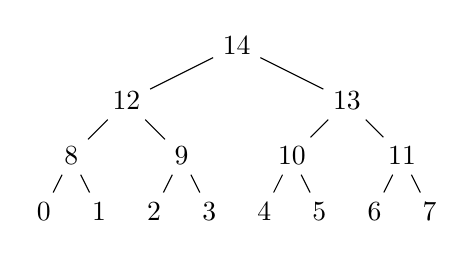
\begin{tikzpicture}[scale=.7]
  \node (0) at (-4,0) {$0$};
  \node (1) at (-3,0) {$1$};
  \node (2) at (-2,0) {$2$};
  \node (3) at (-1,0) {$3$};
    \node (4) at (0,0) {$4$};
  \node (5) at (1,0) {$5$};
  \node (6) at (2,0) {$6$};
  \node (7) at (3,0) {$7$};
  \node (8) at (-3.5,1) {$8$};
  \node (9) at (-1.5,1) {$9$};
  \node (10) at (.5,1) {$10$};
  \node (11) at (2.5,1) {$11$};
    \node (12) at (-2.5,2) {$12$};
  \node (13) at (1.5,2) {$13$};
  \node (14) at (-.5,3) {$14$};
  \draw (0)--(8);
  \draw (1)--(8);
  \draw (2)--(9);
  \draw (3)--(9);
  \draw (4)--(10);
  \draw (5)--(10);
  \draw (6)--(11);
  \draw (7)--(11);
  \draw (8)--(12);
  \draw (9)--(12);
  \draw (10)--(13);
  \draw (11)--(13);
  \draw (12)--(14);
  \draw (13)--(14);
\end{tikzpicture}
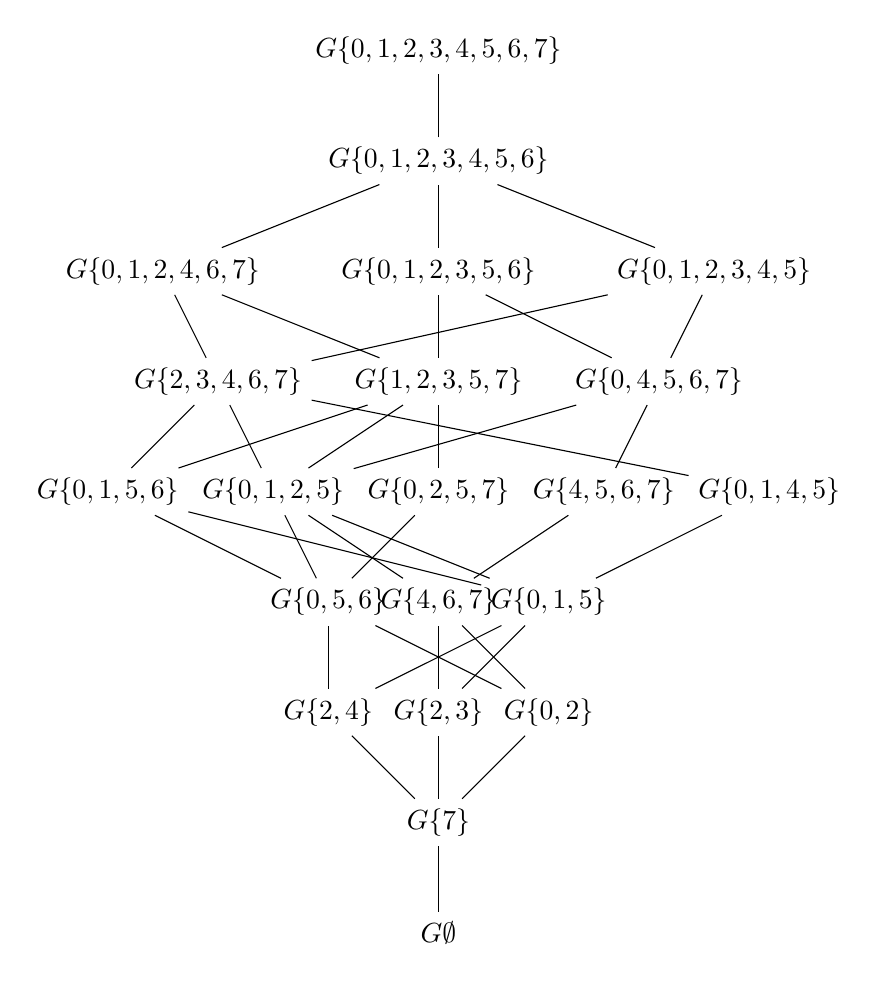
\begin{tikzpicture}[scale=.7]
  \node (0) at (0,-2) {$G\emptyset$};
  
  \node (1) at (0,0) {$G\{7\}$};
  
  \node (2) at (-2,2) {$G\{2,4\}$};
  \node (3) at (0,2) {$G\{2,3\}$};
  \node (4) at (2,2) {$G\{0,2\}$};
  
  \node (5) at (-2,4) {$G\{0,5,6\}$};
  \node (6) at (0,4) {$G\{4,6,7\}$};
  \node (7) at (2,4) {$G\{0,1,5\}$};
  
  \node (8) at (-6,6) {$G\{0,1,5,6\}$};
  \node (9) at (-3,6) {$G\{0,1,2,5\}$};
  \node (10) at (0,6) {$G\{0,2,5,7\}$};
  \node (11) at (3,6) {$G\{4,5,6,7\}$};
  \node (12) at (6,6) {$G\{0,1,4,5\}$};
  
  \node (13) at (-4,8) {$G\{2,3,4,6,7\}$};
  \node (14) at (0,8) {$G\{1,2,3,5,7\}$};
  \node (15) at (4,8) {$G\{0,4,5,6,7\}$};
  
  \node (16) at (-5,10) {$G\{0,1,2,4,6,7\}$};
  \node (17) at (0,10) {$G\{0,1,2,3,5,6\}$};
  \node (18) at (5,10) {$G\{0,1,2,3,4,5\}$};
  
  \node (19) at (0,12) {$G\{0,1,2,3,4,5,6\}$};
  
  \node (20) at (0,14) {$G\{0,1,2,3,4,5,6,7\}$};

  \draw (0) -- (1);
  
  \draw (1) -- (2);
  \draw (1) -- (3);
  \draw (1) -- (4);
  
  \draw (2) -- (5);
  \draw (2) -- (7);
  \draw (3) -- (6);
  \draw (3) -- (7);
  \draw (4) -- (5);
  \draw (4) -- (6);
  \draw (5) -- (8);
  \draw (5) -- (9);
  \draw (5) -- (10);
  \draw (6) -- (9);
  \draw (6) -- (11);
  \draw (7) -- (8);
  \draw (7) -- (9);
  \draw (7) -- (12);
  \draw (8) -- (13);
  \draw (8) -- (14);
  \draw (9) -- (13);
  \draw (9) -- (14);
  \draw (9) -- (15);
  \draw (10) -- (14);
  \draw (11) -- (15);
  \draw (12) -- (13);
  \draw (13) -- (16);
  \draw (13) -- (18);
  \draw (14) -- (16);
  \draw (14) -- (17);
  \draw (15) -- (17);
  \draw (15) -- (18);
  \draw (16) -- (19);
  \draw (17) -- (19);
  \draw (18) -- (19);
  \draw (19) -- (20);
\end{tikzpicture}

\ssec{A Failed Attempt for Showing $\mathcal F^1(B_n/G)$ is unimodal}

In this section, we describe one path we were pursuing in order to show $\mathcal F^1(B_n/G)$ is unimodal. We were attempting to do this by trying to show there were injective order raising maps $U_i:\mathcal F^1(B_n/G)_i \rightarrow \mathcal F^1(B_n/G)_{i+1}.$

We shall now define several maps, so that we can draw a certain commuting diagram in Remark ~\ref{failed_commuting_diagram}


\begin{note}
Let $U_i:P_i \rightarrow P_{i+1}$ be the raising operator for the poset $P.$ Then, we obtain an induced map
\begin{align*}
	U_i \otimes U_{i+1}:P_i\otimes P_{i+1} \rightarrow P_{i+1} \otimes P_{i+1},x \otimes y \mapsto U(x) \otimes U(y).
\end{align*}

We also have the natural inclusions
\begin{align*}
	k_i:\mathcal F^1(P)_i &\rightarrow P_i \otimes P_{i+1},\\
	x\otimes y &\mapsto x\otimes y\\
	k_i^{G\times G}:\mathcal F^1(P/G)_i &\rightarrow (P/G)_i \otimes (P/G)_{i+1},\\
	Gx\otimes Gy &\mapsto Gx\otimes Gy,
\end{align*}
where we have $x \lessdot y$ and $Gx \lessdot Gy.$ The maps above are defined on a basis, and are extended by linearity.

Next, we define the map
\begin{align*}
	j_i:\mathcal (P/G)_i \otimes (P/G)_{i+1} & \rightarrow P_i \otimes P_{i+1},\\
	Gx\otimes Gy &\mapsto \frac{1}{|G|}\sum_{g \in G}^{} gx\otimes \frac{1}{|G|}\sum_{h\in G}^{}hy.
\end{align*}
where $x$ is an arbitrary representative of $Gx$ and $y$ is an arbitrary representative of $Gy$

Then, define the map
\begin{align*}
	p_i: P_i \otimes P_{i+1} &\rightarrow \mathcal (P/G)_i \otimes (P/G)_{i+1},\\
	x\otimes y &\mapsto Gx\otimes Gy.
\end{align*}

Further, define the map 
\begin{align*}
	(U_i \otimes U_{i+1})^{G\times G}:P_i\otimes P_{i+1} &\rightarrow P_{i+1} \otimes P_{i+1},\\
	Gx \otimes Gy &\mapsto p_{i+1}\circ(U_i \otimes U_{i+1})\circ j_i(Gx\otimes Gy).
\end{align*}

We also have the projections inclusions
\begin{align*}
	\pi_i:P_i \otimes P_{i+1} & \rightarrow \mathcal F^1(P)_{i},\\
	x\otimes y &\mapsto  \begin{cases}
	x\otimes y, &\text{ if }x\lessdot y\\
	0 &\text { otherwise}
\end{cases}\\
	\pi_i^{G\times G}: (P/G)_i \otimes (P/G)_{i+1} &\rightarrow\mathcal F^1(P/G)_i,\\
	Gx\otimes Gy &\mapsto \begin{cases}
	Gx\otimes Gy, &\text{ if }Gx\lessdot Gy\\
	0 &\text { otherwise}
\end{cases},
\end{align*}
where we have $x \lessdot y$ and $Gx \lessdot Gy.$ The maps above are defined on a basis, and are extended by linearity.

Finally, denote
\begin{align*}
	\mathcal F^1(U)_i:\mathcal F^1(P)_i &\rightarrow \mathcal F^1(P)_{i+1}\\
	x\otimes y &\mapsto k_i \circ (U \otimes U) \circ \pi_{i+1}(x\otimes y)\\
\mathcal F^1(U)^{G\times G}_i:\mathcal F^1(P/G)_i & \rightarrow \mathcal F^1(P/G)_{i+1}\\
	Gx\otimes Gy &\mapsto k^{G\times G}_i \circ (U \otimes U)^{G\times G} \circ \pi^{G\times G}_{i+1}(Gx\otimes Gy)
\end{align*}
where it is defined above on a basis and we extend to the whole space by linearity.
\end{note}

\begin{rem}
\label{failed_commuting_diagram}
For $i < \frac{n}{2}$ we obtain the following (almost commuting, but $j_{i+1}\circ p_{i+1} \neq \id.$) diagram

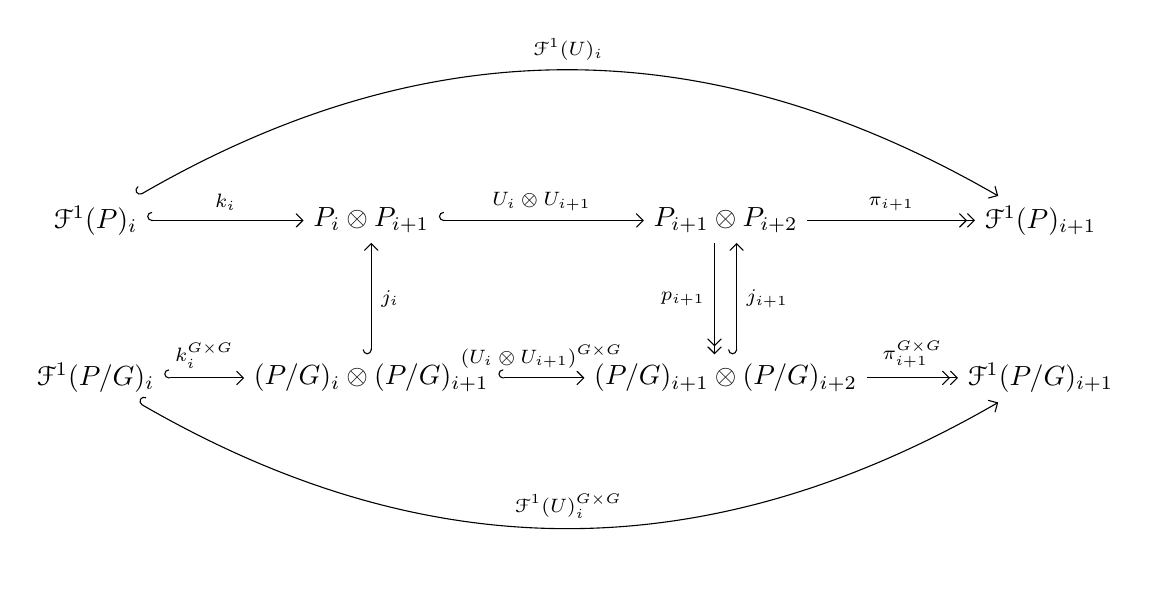
\begin{tikzpicture}[baseline=(current  bounding  box.center)]
\node (a) at (0,0) {$\mathcal F^1(P)_i$};
\node (b) at (3.5,0) {$P_i \otimes P_{i+1}$};
\node (c) at (8,0) {$P_{i+1} \otimes P_{i+2} $};
\node (d) at (12,0) {$\mathcal F^1(P)_{i+1}$};
\node (e) at (0,-2) {$\mathcal F^1(P/G)_i$};
\node (f) at (3.5,-2) {$(P/G)_i \otimes (P/G)_{i+1}$};
\node (g) at (8,-2) {$(P/G)_{i+1} \otimes (P/G)_{i+2} $};
\node (h) at (12,-2) {$\mathcal F^1(P/G)_{i+1}$};
\path[right hook->,font=\scriptsize,>=angle 90] ([xshift= 4pt]g.north) edge node[right] {$j_{i+1}$} ([xshift= 4pt]c.south)
(a) edge node[above]{$k_i$} (b)
(b) edge node[above]{$U_i\otimes U_{i+1}$} (c)
(e) edge node[above]{$k_i^{G\times G}$}(f)
(f) edge node[above] {$(U_i \otimes U_{i+1})^{G\times G}$} (g)
(f) edge node[right] {$j_{i}$} (b)
(a) edge [bend left] node[above] {$\mathcal F^1(U)_i$} (d)
(e) edge [bend right] node[above] {$\mathcal F^1(U)^{G\times G}_i$} (h)
;
\path[->>,font=\scriptsize,>=angle 90]
([xshift= -4pt]c.south) edge node[left] {$p_{i+1}$} ([xshift= -4pt]g.north)
(c) edge node[above] {$\pi_{i+1}$}(d)
(g) edge node[above] {$\pi_{i+1}^{G\times G}$} (h)
;
\end{tikzpicture}


Unfortunately, in general, with the above definitions of the maps, 
$$\ker \left(\pi^{G\times G}_{i+1}\circ p_{i+1}\right) \cap \im((U\otimes U)\circ j_i\circ k^{G\times G}_i)
\not\subset \ker \pi_{i+1} \cap \im((U\otimes U)\circ j_i\circ k^{G\times G}_i).$$
However, if we did have 
$$\ker \left(\pi^{G\times G}_{i+1}\circ p_{i+1}\right) \cap \im((U\otimes U)\circ j_i\circ k^{G\times G}_i)
\subset \ker \pi_{i+1} \cap \im((U\otimes U)\circ j_i\circ k^{G\times G}_i),$$
using the fact that $\mathcal F^1(U)_i,U_i,U_{i+1}$ are all injective, a fairly simple diagram chase would reveal $\mathcal F^1(U)_i^{G\times G}$ is injective. This, in turn, would imply $\mathcal F^1(B_n/G)_i$ is symmetric, unimodal, and sperner.
We have tried several variations on these exact maps, but were never quite able to obtain the desired $\ker \left(\pi^{G\times G}_{i+1}\circ p_{i+1}\right) \cap \im((U\otimes U)\circ j_i\circ k^{G\times G}_i)\subset \ker \pi_{i+1} \cap \im((U\otimes U)\circ j_i\circ k^{G\times G}_i).$
\end{rem}

\bibliography{References}
\bibliographystyle{alpha}


\end{document}